\documentclass[]{article}
\usepackage{lmodern}
\usepackage{amssymb,amsmath}
\usepackage{ifxetex,ifluatex}
\usepackage{fixltx2e} % provides \textsubscript
\ifnum 0\ifxetex 1\fi\ifluatex 1\fi=0 % if pdftex
  \usepackage[T1]{fontenc}
  \usepackage[utf8]{inputenc}
\else % if luatex or xelatex
  \ifxetex
    \usepackage{mathspec}
  \else
    \usepackage{fontspec}
  \fi
  \defaultfontfeatures{Ligatures=TeX,Scale=MatchLowercase}
\fi
% use upquote if available, for straight quotes in verbatim environments
\IfFileExists{upquote.sty}{\usepackage{upquote}}{}
% use microtype if available
\IfFileExists{microtype.sty}{%
\usepackage{microtype}
\UseMicrotypeSet[protrusion]{basicmath} % disable protrusion for tt fonts
}{}
\usepackage[margin=1in]{geometry}
\usepackage{hyperref}
\hypersetup{unicode=true,
            pdftitle={Data 621 Homework 4: Car Insurance},
            pdfauthor={Tommy Jenkins, Violeta Stoyanova, Todd Weigel, Peter Kowalchuk, Eleanor R-Secoquian, Anthony Pagan},
            pdfborder={0 0 0},
            breaklinks=true}
\urlstyle{same}  % don't use monospace font for urls
\usepackage{color}
\usepackage{fancyvrb}
\newcommand{\VerbBar}{|}
\newcommand{\VERB}{\Verb[commandchars=\\\{\}]}
\DefineVerbatimEnvironment{Highlighting}{Verbatim}{commandchars=\\\{\}}
% Add ',fontsize=\small' for more characters per line
\usepackage{framed}
\definecolor{shadecolor}{RGB}{248,248,248}
\newenvironment{Shaded}{\begin{snugshade}}{\end{snugshade}}
\newcommand{\AlertTok}[1]{\textcolor[rgb]{0.94,0.16,0.16}{#1}}
\newcommand{\AnnotationTok}[1]{\textcolor[rgb]{0.56,0.35,0.01}{\textbf{\textit{#1}}}}
\newcommand{\AttributeTok}[1]{\textcolor[rgb]{0.77,0.63,0.00}{#1}}
\newcommand{\BaseNTok}[1]{\textcolor[rgb]{0.00,0.00,0.81}{#1}}
\newcommand{\BuiltInTok}[1]{#1}
\newcommand{\CharTok}[1]{\textcolor[rgb]{0.31,0.60,0.02}{#1}}
\newcommand{\CommentTok}[1]{\textcolor[rgb]{0.56,0.35,0.01}{\textit{#1}}}
\newcommand{\CommentVarTok}[1]{\textcolor[rgb]{0.56,0.35,0.01}{\textbf{\textit{#1}}}}
\newcommand{\ConstantTok}[1]{\textcolor[rgb]{0.00,0.00,0.00}{#1}}
\newcommand{\ControlFlowTok}[1]{\textcolor[rgb]{0.13,0.29,0.53}{\textbf{#1}}}
\newcommand{\DataTypeTok}[1]{\textcolor[rgb]{0.13,0.29,0.53}{#1}}
\newcommand{\DecValTok}[1]{\textcolor[rgb]{0.00,0.00,0.81}{#1}}
\newcommand{\DocumentationTok}[1]{\textcolor[rgb]{0.56,0.35,0.01}{\textbf{\textit{#1}}}}
\newcommand{\ErrorTok}[1]{\textcolor[rgb]{0.64,0.00,0.00}{\textbf{#1}}}
\newcommand{\ExtensionTok}[1]{#1}
\newcommand{\FloatTok}[1]{\textcolor[rgb]{0.00,0.00,0.81}{#1}}
\newcommand{\FunctionTok}[1]{\textcolor[rgb]{0.00,0.00,0.00}{#1}}
\newcommand{\ImportTok}[1]{#1}
\newcommand{\InformationTok}[1]{\textcolor[rgb]{0.56,0.35,0.01}{\textbf{\textit{#1}}}}
\newcommand{\KeywordTok}[1]{\textcolor[rgb]{0.13,0.29,0.53}{\textbf{#1}}}
\newcommand{\NormalTok}[1]{#1}
\newcommand{\OperatorTok}[1]{\textcolor[rgb]{0.81,0.36,0.00}{\textbf{#1}}}
\newcommand{\OtherTok}[1]{\textcolor[rgb]{0.56,0.35,0.01}{#1}}
\newcommand{\PreprocessorTok}[1]{\textcolor[rgb]{0.56,0.35,0.01}{\textit{#1}}}
\newcommand{\RegionMarkerTok}[1]{#1}
\newcommand{\SpecialCharTok}[1]{\textcolor[rgb]{0.00,0.00,0.00}{#1}}
\newcommand{\SpecialStringTok}[1]{\textcolor[rgb]{0.31,0.60,0.02}{#1}}
\newcommand{\StringTok}[1]{\textcolor[rgb]{0.31,0.60,0.02}{#1}}
\newcommand{\VariableTok}[1]{\textcolor[rgb]{0.00,0.00,0.00}{#1}}
\newcommand{\VerbatimStringTok}[1]{\textcolor[rgb]{0.31,0.60,0.02}{#1}}
\newcommand{\WarningTok}[1]{\textcolor[rgb]{0.56,0.35,0.01}{\textbf{\textit{#1}}}}
\usepackage{longtable,booktabs}
\usepackage{graphicx,grffile}
\makeatletter
\def\maxwidth{\ifdim\Gin@nat@width>\linewidth\linewidth\else\Gin@nat@width\fi}
\def\maxheight{\ifdim\Gin@nat@height>\textheight\textheight\else\Gin@nat@height\fi}
\makeatother
% Scale images if necessary, so that they will not overflow the page
% margins by default, and it is still possible to overwrite the defaults
% using explicit options in \includegraphics[width, height, ...]{}
\setkeys{Gin}{width=\maxwidth,height=\maxheight,keepaspectratio}
\IfFileExists{parskip.sty}{%
\usepackage{parskip}
}{% else
\setlength{\parindent}{0pt}
\setlength{\parskip}{6pt plus 2pt minus 1pt}
}
\setlength{\emergencystretch}{3em}  % prevent overfull lines
\providecommand{\tightlist}{%
  \setlength{\itemsep}{0pt}\setlength{\parskip}{0pt}}
\setcounter{secnumdepth}{0}
% Redefines (sub)paragraphs to behave more like sections
\ifx\paragraph\undefined\else
\let\oldparagraph\paragraph
\renewcommand{\paragraph}[1]{\oldparagraph{#1}\mbox{}}
\fi
\ifx\subparagraph\undefined\else
\let\oldsubparagraph\subparagraph
\renewcommand{\subparagraph}[1]{\oldsubparagraph{#1}\mbox{}}
\fi

%%% Use protect on footnotes to avoid problems with footnotes in titles
\let\rmarkdownfootnote\footnote%
\def\footnote{\protect\rmarkdownfootnote}

%%% Change title format to be more compact
\usepackage{titling}

% Create subtitle command for use in maketitle
\providecommand{\subtitle}[1]{
  \posttitle{
    \begin{center}\large#1\end{center}
    }
}

\setlength{\droptitle}{-2em}

  \title{Data 621 Homework 4: Car Insurance}
    \pretitle{\vspace{\droptitle}\centering\huge}
  \posttitle{\par}
    \author{Tommy Jenkins, Violeta Stoyanova, Todd Weigel, Peter Kowalchuk, Eleanor
R-Secoquian, Anthony Pagan}
    \preauthor{\centering\large\emph}
  \postauthor{\par}
      \predate{\centering\large\emph}
  \postdate{\par}
    \date{November 15, 2019}

\usepackage{booktabs}
\usepackage{longtable}
\usepackage{array}
\usepackage{multirow}
\usepackage{wrapfig}
\usepackage{float}
\usepackage{colortbl}
\usepackage{pdflscape}
\usepackage{tabu}
\usepackage{threeparttable}
\usepackage{threeparttablex}
\usepackage[normalem]{ulem}
\usepackage{makecell}
\usepackage{xcolor}

\begin{document}
\maketitle

\hypertarget{overview}{%
\section{OVERVIEW}\label{overview}}

In this homework assignment, we will explore, analyze and model a data
set containing approximately 8000 records representing a customer at an
auto insurance company. Each record has two response variables. The
first response variable, TARGET\_FLAG, is a 1 or a 0. A ``1'' means that
the person was in a car crash. A zero means that the person was not in a
car crash. The second response variable is TARGET\_AMT. This value is
zero if the person did not crash their car. But if they did crash their
car, this number will be a value greater than zero representing the cost
of the crash.

\hypertarget{objective}{%
\subsection{Objective:}\label{objective}}

Our objective is to build multiple linear regression and binary logistic
regression models on the training data to predict the probability that a
person will crash their car and also the amount of money it will cost if
the person does crash their car.

\hypertarget{data-exploration}{%
\section{DATA EXPLORATION}\label{data-exploration}}

\hypertarget{data-summary}{%
\subsection{Data Summary}\label{data-summary}}

The dataset consists of two data files: training and evaluation. The
training dataset contains 26 columns, while the evaluation dataset
contains 26. The evaluation dataset is missing columns which represent
our response variables, respectively whether the person was in a car
crash and the cost of the car crash if the person was in an accident. We
will start by exploring the training data set since it will be the one
used to generate the models.

The columns in the data set are:\\
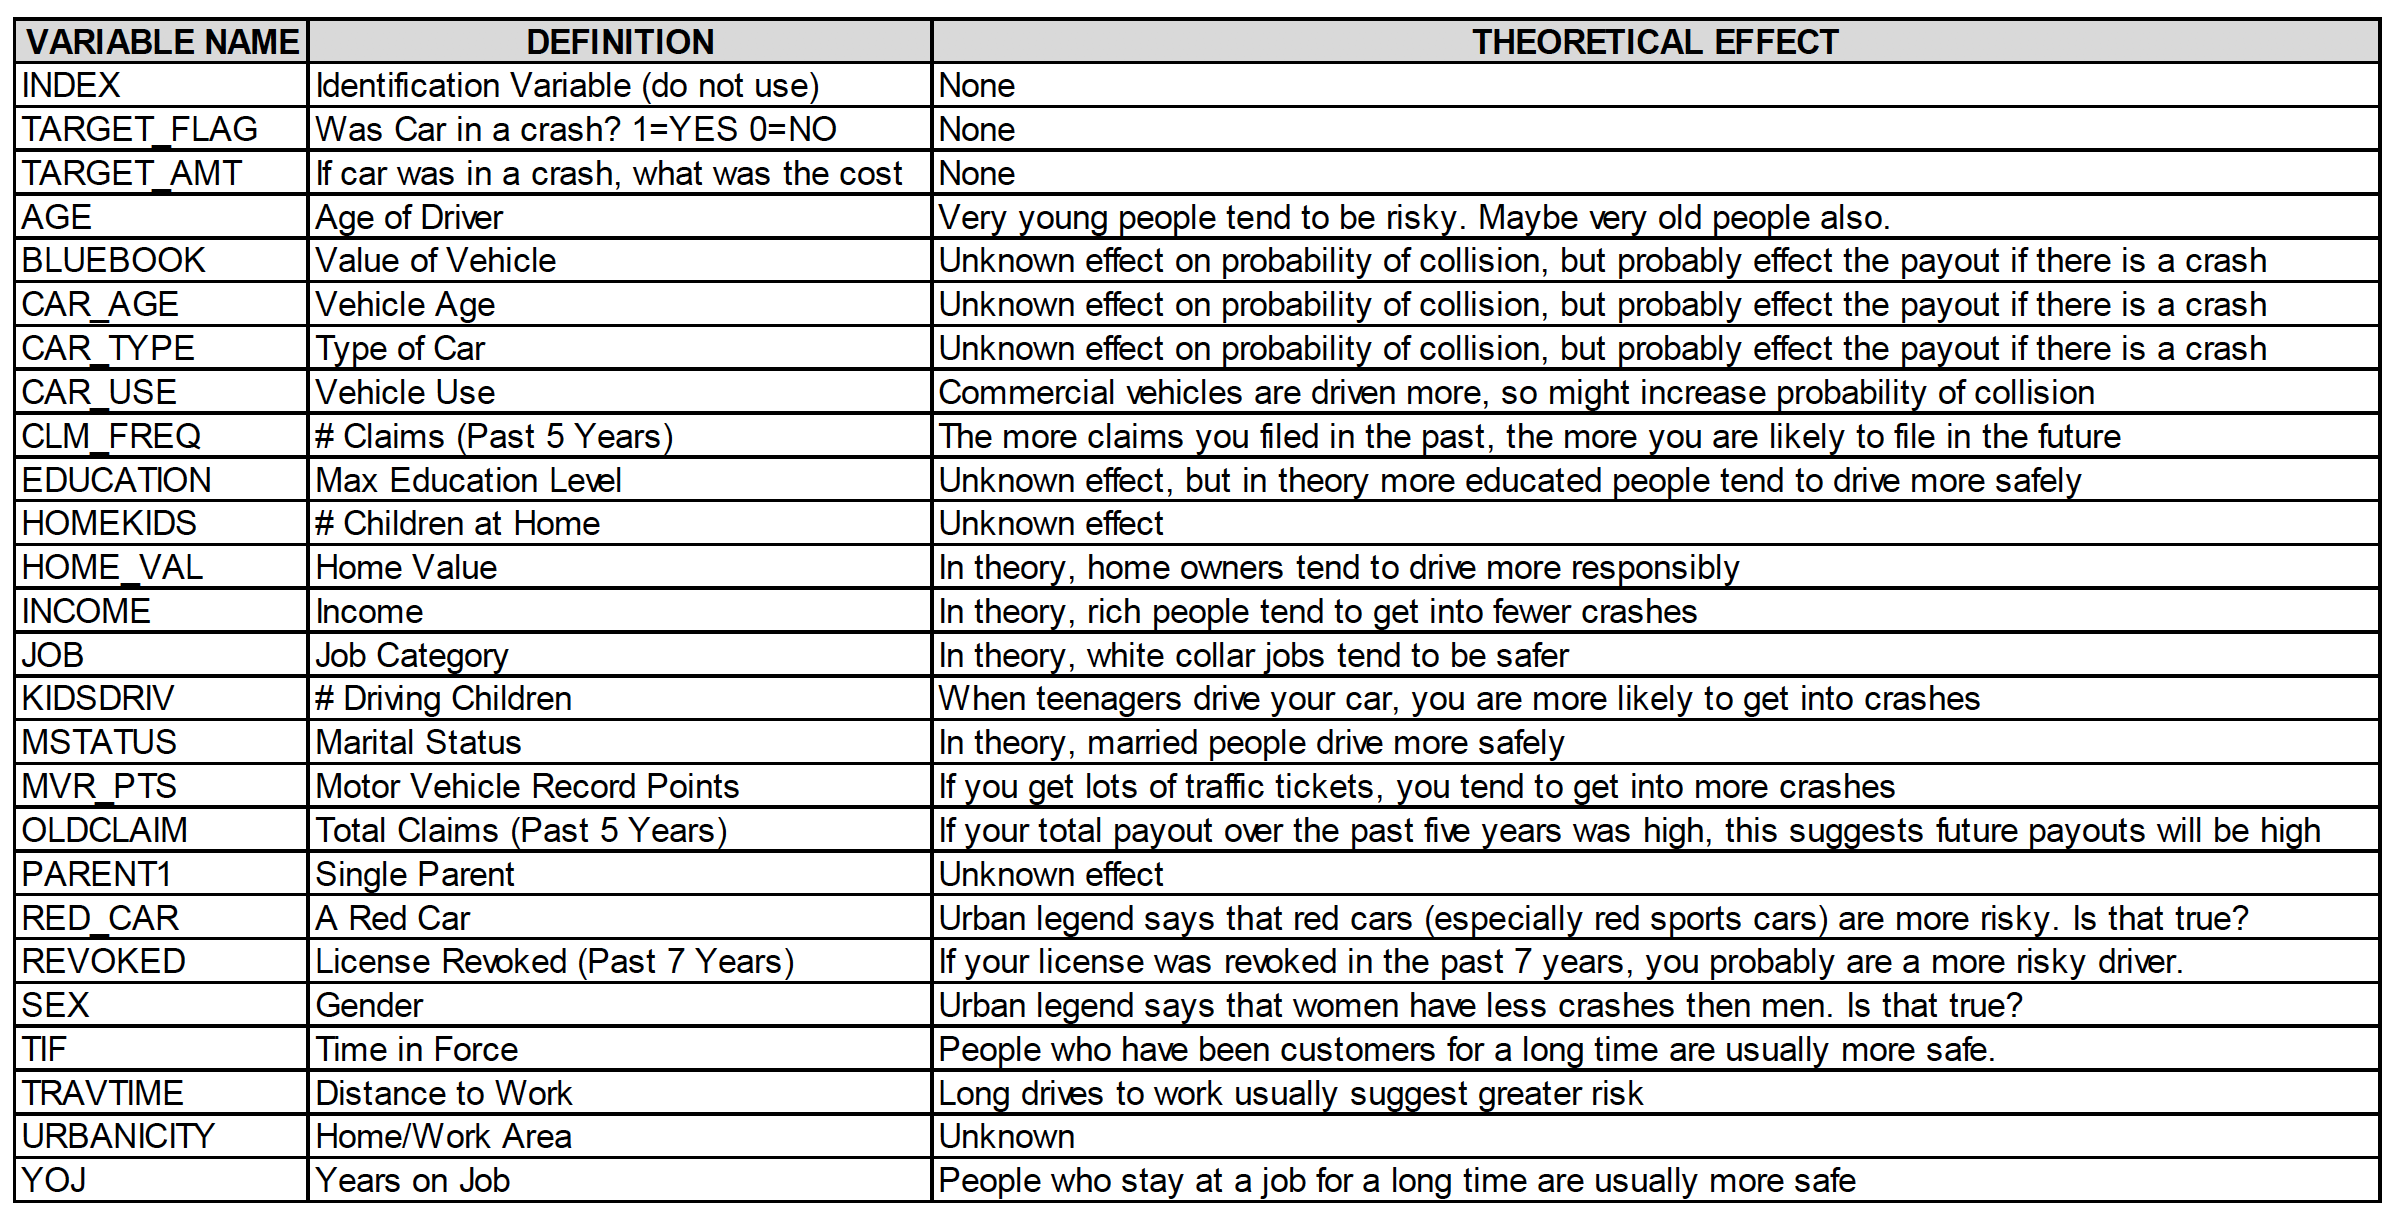
\includegraphics{dataTable.png}

\hypertarget{missing-data}{%
\subsection{Missing Data}\label{missing-data}}

An important aspect of any dataset is to determine how much, if any,
data is missing. We look at all the variables to see which if any have
missing data. We look at the basic descriptive statistics as well as the
missing data and percentages.

We start by looking at the dataset as a whole and determine how many
complete rows, that is rows with data for all predictors, do we have.

\begin{verbatim}
##    Mode   FALSE    TRUE 
## logical    2116    6045
\end{verbatim}

With these results, if we remove all rows with incomplete rows, there
will be a total of 6045 rows out of 8161 .If we eliminate all
non-complete rows and keep only rows with data for all the predictors in
the dataset, our new dataset will results in 74\% of the total dataset.
We create a subset of data with complete cases only to use later in our
analysis.

\begin{verbatim}
## Observations: 6,045
## Variables: 26
## $ INDEX       <int> 1, 2, 4, 7, 12, 13, 14, 15, 16, 19, 20, 22, 23, 24...
## $ TARGET_FLAG <int> 0, 0, 0, 1, 1, 0, 1, 0, 0, 1, 0, 0, 0, 0, 1, 0, 0,...
## $ TARGET_AMT  <dbl> 0.000, 0.000, 0.000, 2946.000, 2501.000, 0.000, 60...
## $ KIDSDRIV    <int> 0, 0, 0, 0, 0, 0, 0, 0, 0, 0, 0, 0, 0, 0, 0, 0, 0,...
## $ AGE         <int> 60, 43, 35, 34, 34, 50, 53, 43, 55, 45, 39, 42, 34...
## $ HOMEKIDS    <int> 0, 0, 1, 1, 0, 0, 0, 0, 0, 0, 3, 0, 3, 2, 1, 0, 0,...
## $ YOJ         <int> 11, 11, 10, 12, 10, 7, 14, 5, 11, 0, 12, 11, 13, 1...
## $ INCOME      <fct> "$67,349", "$91,449", "$16,039", "$125,301", "$62,...
## $ PARENT1     <fct> No, No, No, Yes, No, No, No, No, No, No, Yes, No, ...
## $ HOME_VAL    <fct> "$0", "$257,252", "$124,191", "$0", "$0", "$0", "$...
## $ MSTATUS     <fct> z_No, z_No, Yes, z_No, z_No, z_No, z_No, Yes, Yes,...
## $ SEX         <fct> M, M, z_F, z_F, z_F, M, z_F, z_F, M, z_F, z_F, M, ...
## $ EDUCATION   <fct> PhD, z_High School, z_High School, Bachelors, Bach...
## $ JOB         <fct> Professional, z_Blue Collar, Clerical, z_Blue Coll...
## $ TRAVTIME    <int> 14, 22, 5, 46, 34, 48, 15, 36, 25, 48, 43, 42, 27,...
## $ CAR_USE     <fct> Private, Commercial, Private, Commercial, Private,...
## $ BLUEBOOK    <fct> "$14,230", "$14,940", "$4,010", "$17,430", "$11,20...
## $ TIF         <int> 11, 1, 4, 1, 1, 7, 1, 7, 7, 1, 6, 6, 7, 4, 6, 6, 1...
## $ CAR_TYPE    <fct> Minivan, Minivan, z_SUV, Sports Car, z_SUV, Van, S...
## $ RED_CAR     <fct> yes, yes, no, no, no, no, no, no, yes, no, no, no,...
## $ OLDCLAIM    <fct> "$4,461", "$0", "$38,690", "$0", "$0", "$0", "$0",...
## $ CLM_FREQ    <int> 2, 0, 2, 0, 0, 0, 0, 0, 2, 0, 0, 0, 0, 0, 2, 1, 0,...
## $ REVOKED     <fct> No, No, No, No, No, No, No, No, Yes, No, No, No, N...
## $ MVR_PTS     <int> 3, 0, 3, 0, 0, 1, 0, 0, 3, 3, 0, 0, 0, 0, 0, 5, 1,...
## $ CAR_AGE     <int> 18, 1, 10, 7, 1, 17, 11, 1, 9, 5, 13, 16, 20, 7, 1...
## $ URBANICITY  <fct> Highly Urban/ Urban, Highly Urban/ Urban, Highly U...
\end{verbatim}

But we can also look at what specific predictors are missing in our
dataset. If we do this we can see how there is much more data available,
as we find only 5 predictors with missing data. Data missing for these
predictors also only accounts for less than 7\% of the respective
predictors total.

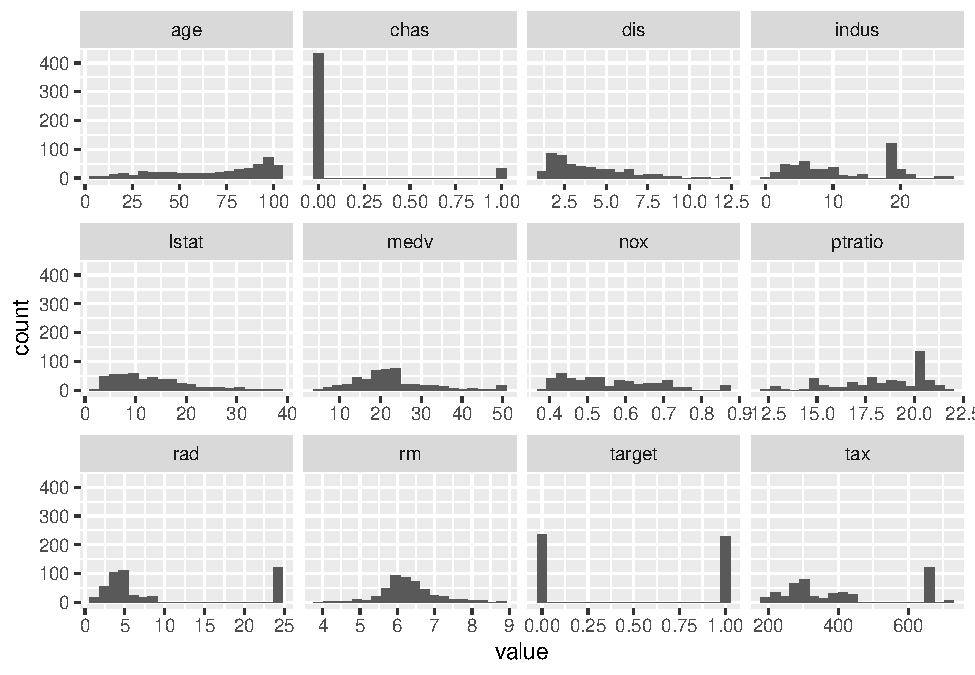
\includegraphics{Data621-Group1-HW4-Final_files/figure-latex/unnamed-chunk-7-1.pdf}

We look closer at the missing data and look at the intersection of
predictors with missing data. We find that the bulk of the missing data
is for predictors with no intersection with other missing predictor
data.

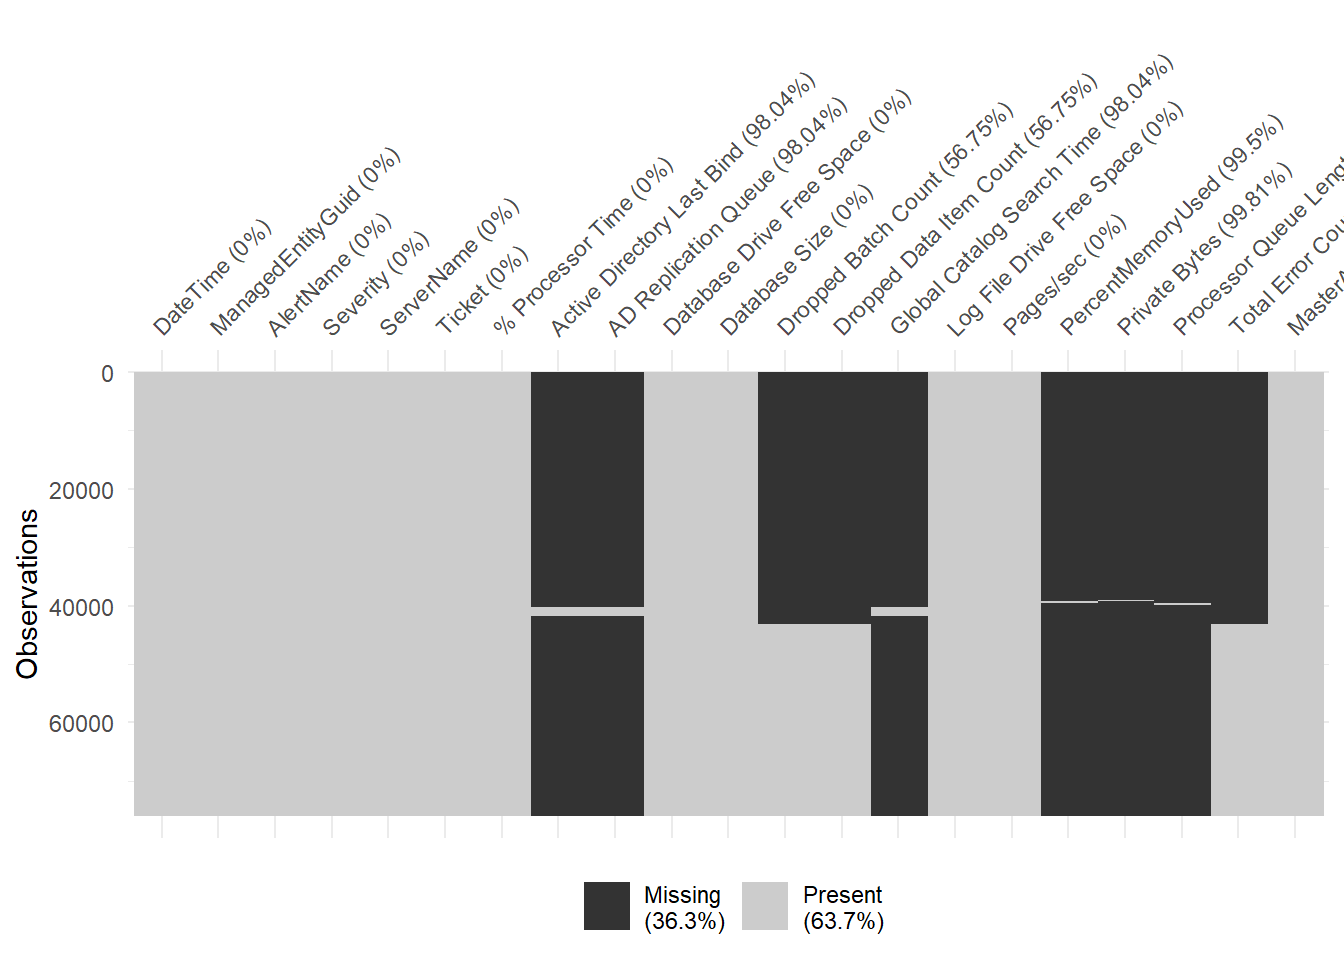
\includegraphics{Data621-Group1-HW4-Final_files/figure-latex/unnamed-chunk-8-1.pdf}

Having this detail in missing data might be of importance when looking
at models. In the next Data Preparation section we will handle these
missing cases and build a data set with data for all predictors in all
rows.

\hypertarget{data-exploration-1}{%
\subsection{Data Exploration}\label{data-exploration-1}}

Using TARGET\_FLAG as response variables we confirm when TARGET\_FLAG is
1 TARGET\_AMOUNT \textgreater0 and when TARGET\_FLAG is 0 when
TARGET\_AMOUNT = 0

\begin{Shaded}
\begin{Highlighting}[]
\KeywordTok{nrow}\NormalTok{(}\KeywordTok{subset}\NormalTok{(InsTrain,TARGET_FLAG }\OperatorTok{==}\StringTok{ }\DecValTok{0}\NormalTok{))}
\end{Highlighting}
\end{Shaded}

\begin{verbatim}
## [1] 6008
\end{verbatim}

\begin{Shaded}
\begin{Highlighting}[]
\KeywordTok{nrow}\NormalTok{(}\KeywordTok{subset}\NormalTok{(InsTrain,TARGET_AMT }\OperatorTok{==}\StringTok{ }\DecValTok{0}\NormalTok{))}
\end{Highlighting}
\end{Shaded}

\begin{verbatim}
## [1] 6008
\end{verbatim}

\begin{Shaded}
\begin{Highlighting}[]
\KeywordTok{nrow}\NormalTok{(}\KeywordTok{subset}\NormalTok{(InsTrain,TARGET_FLAG }\OperatorTok{>}\StringTok{ }\DecValTok{0}\NormalTok{))}
\end{Highlighting}
\end{Shaded}

\begin{verbatim}
## [1] 2153
\end{verbatim}

\begin{Shaded}
\begin{Highlighting}[]
\KeywordTok{nrow}\NormalTok{(}\KeywordTok{subset}\NormalTok{(InsTrain,TARGET_AMT }\OperatorTok{>}\StringTok{ }\DecValTok{0}\NormalTok{))}
\end{Highlighting}
\end{Shaded}

\begin{verbatim}
## [1] 2153
\end{verbatim}

A glimpse of the data shows that the following columns should be
integers and not Factors:

\begin{itemize}
\tightlist
\item
  INCOME
\item
  HOME\_VAL
\item
  BLUEBOOK
\item
  OLDCLAIM
\end{itemize}

We display and view data with all cases and only complete cases

\begin{verbatim}
## INCOME PARENT1 HOME_VAL MSTATUS SEX EDUCATION JOB CAR_USE BLUEBOOK CAR_TYPE RED_CAR OLDCLAIM REVOKED URBANICITY
\end{verbatim}

\begin{verbatim}
## Observations: 8,161
## Variables: 26
## $ INDEX       <int> 1, 2, 4, 5, 6, 7, 8, 11, 12, 13, 14, 15, 16, 17, 1...
## $ TARGET_FLAG <int> 0, 0, 0, 0, 0, 1, 0, 1, 1, 0, 1, 0, 0, 1, 1, 0, 0,...
## $ TARGET_AMT  <dbl> 0.000, 0.000, 0.000, 0.000, 0.000, 2946.000, 0.000...
## $ KIDSDRIV    <int> 0, 0, 0, 0, 0, 0, 0, 1, 0, 0, 0, 0, 0, 0, 0, 0, 0,...
## $ AGE         <int> 60, 43, 35, 51, 50, 34, 54, 37, 34, 50, 53, 43, 55...
## $ HOMEKIDS    <int> 0, 0, 1, 0, 0, 1, 0, 2, 0, 0, 0, 0, 0, 0, 0, 3, 0,...
## $ YOJ         <int> 11, 11, 10, 14, NA, 12, NA, NA, 10, 7, 14, 5, 11, ...
## $ INCOME      <fct> "$67,349", "$91,449", "$16,039", NA, "$114,986", "...
## $ PARENT1     <fct> No, No, No, No, No, Yes, No, No, No, No, No, No, N...
## $ HOME_VAL    <fct> "$0", "$257,252", "$124,191", "$306,251", "$243,92...
## $ MSTATUS     <fct> z_No, z_No, Yes, Yes, Yes, z_No, Yes, Yes, z_No, z...
## $ SEX         <fct> M, M, z_F, M, z_F, z_F, z_F, M, z_F, M, z_F, z_F, ...
## $ EDUCATION   <fct> PhD, z_High School, z_High School, <High School, P...
## $ JOB         <fct> Professional, z_Blue Collar, Clerical, z_Blue Coll...
## $ TRAVTIME    <int> 14, 22, 5, 32, 36, 46, 33, 44, 34, 48, 15, 36, 25,...
## $ CAR_USE     <fct> Private, Commercial, Private, Private, Private, Co...
## $ BLUEBOOK    <fct> "$14,230", "$14,940", "$4,010", "$15,440", "$18,00...
## $ TIF         <int> 11, 1, 4, 7, 1, 1, 1, 1, 1, 7, 1, 7, 7, 6, 1, 6, 6...
## $ CAR_TYPE    <fct> Minivan, Minivan, z_SUV, Minivan, z_SUV, Sports Ca...
## $ RED_CAR     <fct> yes, yes, no, yes, no, no, no, yes, no, no, no, no...
## $ OLDCLAIM    <fct> "$4,461", "$0", "$38,690", "$0", "$19,217", "$0", ...
## $ CLM_FREQ    <int> 2, 0, 2, 0, 2, 0, 0, 1, 0, 0, 0, 0, 2, 0, 0, 0, 0,...
## $ REVOKED     <fct> No, No, No, No, Yes, No, No, Yes, No, No, No, No, ...
## $ MVR_PTS     <int> 3, 0, 3, 0, 3, 0, 0, 10, 0, 1, 0, 0, 3, 3, 3, 0, 0...
## $ CAR_AGE     <int> 18, 1, 10, 6, 17, 7, 1, 7, 1, 17, 11, 1, 9, 10, 5,...
## $ URBANICITY  <fct> Highly Urban/ Urban, Highly Urban/ Urban, Highly U...
\end{verbatim}

We use Sapply function to review which columns have NA Values. It
display columns and percent of values that are missing.

\begin{verbatim}
##       INDEX TARGET_FLAG  TARGET_AMT    KIDSDRIV         AGE    HOMEKIDS 
##         0.0         0.0         0.0         0.0         0.1         0.0 
##         YOJ      INCOME     PARENT1    HOME_VAL     MSTATUS         SEX 
##         5.6         5.5         0.0         5.7         0.0         0.0 
##   EDUCATION         JOB    TRAVTIME     CAR_USE    BLUEBOOK         TIF 
##         0.0         6.4         0.0         0.0         0.0         0.0 
##    CAR_TYPE     RED_CAR    OLDCLAIM    CLM_FREQ     REVOKED     MVR_PTS 
##         0.0         0.0         0.0         0.0         0.0         0.0 
##     CAR_AGE  URBANICITY 
##         6.2         0.0
\end{verbatim}

\hypertarget{data-preparation}{%
\subsection{Data Preparation}\label{data-preparation}}

As revealed earlier there were a list of columns that we factors that
should be integers. We start by converting the columns to numeric.

\begin{verbatim}
## Observations: 8,161
## Variables: 4
## $ INCOME   <fct> "$67,349", "$91,449", "$16,039", NA, "$114,986", "$12...
## $ HOME_VAL <fct> "$0", "$257,252", "$124,191", "$306,251", "$243,925",...
## $ BLUEBOOK <fct> "$14,230", "$14,940", "$4,010", "$15,440", "$18,000",...
## $ OLDCLAIM <fct> "$4,461", "$0", "$38,690", "$0", "$19,217", "$0", "$0...
## Observations: 8,161
## Variables: 4
## $ INCOME   <int> 67349, 91449, 16039, NA, 114986, 125301, 18755, 10796...
## $ HOME_VAL <int> 0, 257252, 124191, 306251, 243925, 0, NA, 333680, 0, ...
## $ BLUEBOOK <int> 14230, 14940, 4010, 15440, 18000, 17430, 8780, 16970,...
## $ OLDCLAIM <int> 4461, 0, 38690, 0, 19217, 0, 0, 2374, 0, 0, 0, 0, 502...
\end{verbatim}

Both boxplot and summary stats with the square root transform of
Home\_val and Income to confirm we can use median or mean values to
replace NA values if we chose.

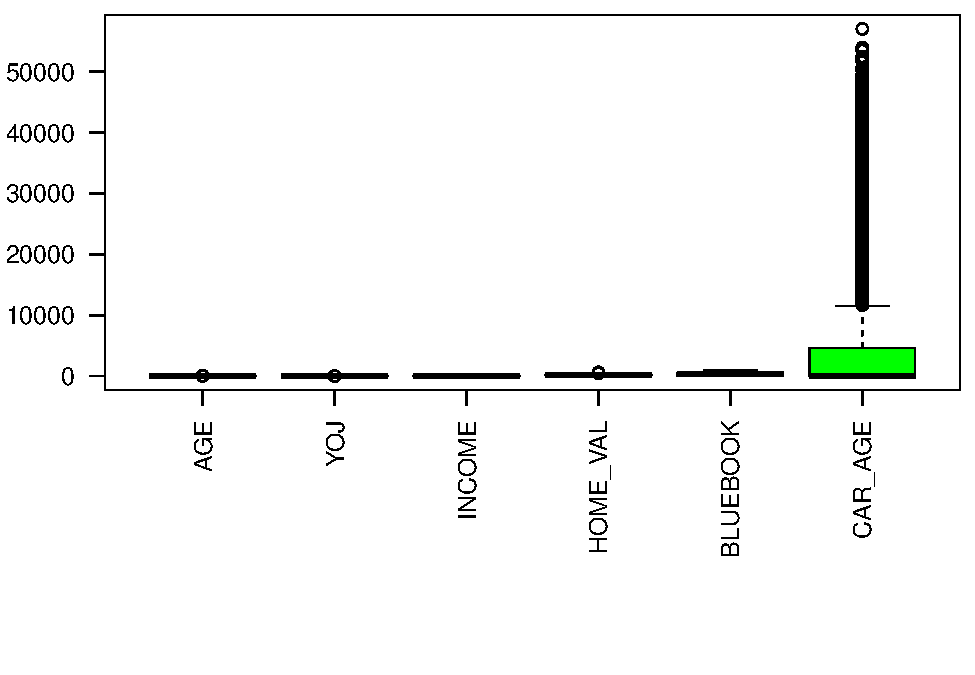
\includegraphics{Data621-Group1-HW4-Final_files/figure-latex/unnamed-chunk-13-1.pdf}

\begin{verbatim}
##          vars    n      mean       sd median   trimmed      mad   min
## AGE         1 8155     44.79     8.63     45     44.83     8.90    16
## YOJ         2 7707     10.50     4.09     11     11.07     2.97     0
## INCOME      3 7101  67258.94 45810.25  58438  61952.41 39533.53     5
## HOME_VAL    4 5403 220620.68 96145.72 206692 211487.81 85498.58 50223
## CAR_AGE     5 7651      8.33     5.70      8      7.96     7.41    -3
##             max  range  skew kurtosis      se
## AGE          81     65 -0.03    -0.06    0.10
## YOJ          23     23 -1.20     1.18    0.05
## INCOME   367030 367025  1.30     2.50  543.63
## HOME_VAL 885282 835059  1.09     1.97 1308.01
## CAR_AGE      28     31  0.28    -0.75    0.07
\end{verbatim}

We next replace all NA values with mean values for cases that are
missing values and rerun sapply function to confirm there are no longer
any missing values.

\begin{verbatim}
##       INDEX TARGET_FLAG  TARGET_AMT    KIDSDRIV         AGE    HOMEKIDS 
##         0.0         0.0         0.0         0.0         0.1         0.0 
##         YOJ      INCOME     PARENT1    HOME_VAL     MSTATUS         SEX 
##         5.6        13.0         0.0        33.8         0.0         0.0 
##   EDUCATION         JOB    TRAVTIME     CAR_USE    BLUEBOOK         TIF 
##         0.0         6.4         0.0         0.0         0.0         0.0 
##    CAR_TYPE     RED_CAR    OLDCLAIM    CLM_FREQ     REVOKED     MVR_PTS 
##         0.0         0.0         0.0         0.0         0.0         0.0 
##     CAR_AGE  URBANICITY 
##         6.2         0.0
\end{verbatim}

\begin{verbatim}
##      Clerical        Doctor    Home Maker        Lawyer       Manager 
##          1271           246           641           835           988 
##  Professional       Student z_Blue Collar          NA's 
##          1117           712          1825           526
\end{verbatim}

\begin{verbatim}
## [1] 6
\end{verbatim}

\begin{verbatim}
##      Clerical        Doctor    Home Maker        Lawyer       Manager 
##          1271           246           641           835           988 
##  Professional       Student z_Blue Collar 
##          1117           712          2351
\end{verbatim}

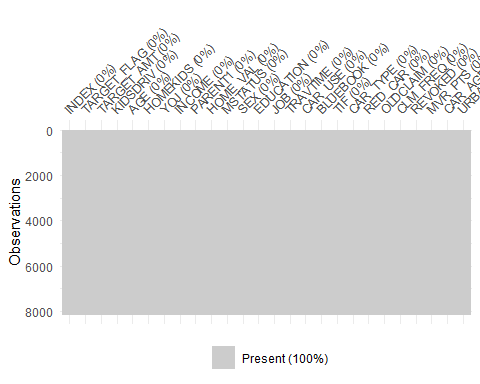
\includegraphics{Data621-Group1-HW4-Final_files/figure-latex/unnamed-chunk-15-1.pdf}

\begin{verbatim}
##          vars    n      mean       sd    median   trimmed      mad   min
## AGE         1 8161     44.79     8.62     45.00     44.83     8.90    16
## YOJ         2 8161     10.50     3.98     11.00     11.05     2.97     0
## INCOME      3 8161  67258.94 42731.37  66367.00  62497.52 36362.25     5
## HOME_VAL    4 8161 220620.68 78227.99 220620.68 214305.03 41344.79 50223
## CAR_AGE     5 8161      8.33     5.52      8.33      7.98     5.44    -3
##             max  range  skew kurtosis     se
## AGE          81     65 -0.03    -0.06   0.10
## YOJ          23     23 -1.24     1.42   0.04
## INCOME   367030 367025  1.40     3.32 473.02
## HOME_VAL 885282 835059  1.34     4.50 865.95
## CAR_AGE      28     31  0.29    -0.60   0.06
\end{verbatim}

We have this way derived a dataset with no missing values. We can use
this set of data for our modeling design. We chose to work with this
data as opposed to the first ``complete'' set in which rows with missing
data were eliminated.

\hypertarget{build-model}{%
\section{Build Model}\label{build-model}}

Modeling design will be divided in two phases. First we will design a
model to predict if the person is in a car crash, that is predict
TARGET\_FLAG. In a second phase, we will predict TARGET\_AMT, the cost
of the crash.

\hypertarget{target_flag-modeling}{%
\subsection{TARGET\_FLAG Modeling}\label{target_flag-modeling}}

This response variable being binary, o or 1, we will be looking at
logistic regression models to find a good fit. We will start with a
naive model with all the predictors included as a baseline. First
approach will be to simply the model by reducing the predictors used. We
will look at several model metrics such as AIC, BIC. We will also
include confusion tables and ROC plot to better understand each model.

\textbf{Model 1: all predictors}

We start out with a straightforward logit logistical regression with all
predictors included. As a note, we need to make sure we do not include
the TARGET\_AMT responce variable in our model as a predictor.

\begin{verbatim}
## 
## Call:
## glm(formula = TARGET_FLAG ~ . - INDEX - TARGET_AMT, family = binomial(link = "logit"), 
##     data = InsTrain)
## 
## Deviance Residuals: 
##     Min       1Q   Median       3Q      Max  
## -2.5548  -0.7184  -0.4032   0.6346   3.1472  
## 
## Coefficients:
##                                   Estimate Std. Error z value Pr(>|z|)    
## (Intercept)                     -4.750e-01  2.748e-01  -1.728 0.083915 .  
## KIDSDRIV                         3.847e-01  6.101e-02   6.306 2.87e-10 ***
## AGE                             -8.588e-04  4.011e-03  -0.214 0.830483    
## HOMEKIDS                         5.680e-02  3.720e-02   1.527 0.126829    
## YOJ                             -1.914e-02  8.888e-03  -2.154 0.031261 *  
## INCOME                          -2.155e-06  1.162e-06  -1.855 0.063585 .  
## PARENT1Yes                       3.795e-01  1.095e-01   3.467 0.000526 ***
## HOME_VAL                        -9.005e-07  5.908e-07  -1.524 0.127471    
## MSTATUSz_No                      6.329e-01  7.272e-02   8.703  < 2e-16 ***
## SEXz_F                          -7.739e-02  1.118e-01  -0.692 0.488791    
## EDUCATIONBachelors              -4.599e-01  1.144e-01  -4.018 5.86e-05 ***
## EDUCATIONMasters                -5.141e-01  1.532e-01  -3.357 0.000789 ***
## EDUCATIONPhD                    -4.617e-01  1.880e-01  -2.456 0.014063 *  
## EDUCATIONz_High School          -1.365e-02  9.467e-02  -0.144 0.885335    
## JOBDoctor                       -7.034e-01  2.656e-01  -2.648 0.008092 ** 
## JOBHome Maker                   -6.625e-02  1.425e-01  -0.465 0.642047    
## JOBLawyer                       -1.851e-01  1.616e-01  -1.146 0.251943    
## JOBManager                      -9.248e-01  1.356e-01  -6.822 8.98e-12 ***
## JOBProfessional                 -2.485e-01  1.215e-01  -2.045 0.040901 *  
## JOBStudent                      -2.503e-03  1.301e-01  -0.019 0.984651    
## JOBz_Blue Collar                -1.727e-01  1.049e-01  -1.645 0.099934 .  
## TRAVTIME                         1.464e-02  1.878e-03   7.791 6.64e-15 ***
## CAR_USEPrivate                  -7.768e-01  9.085e-02  -8.550  < 2e-16 ***
## BLUEBOOK                        -2.204e-05  5.235e-06  -4.210 2.56e-05 ***
## TIF                             -5.561e-02  7.333e-03  -7.583 3.37e-14 ***
## CAR_TYPEPanel Truck              4.823e-01  1.577e-01   3.058 0.002230 ** 
## CAR_TYPEPickup                   5.241e-01  9.983e-02   5.250 1.52e-07 ***
## CAR_TYPESports Car               1.022e+00  1.297e-01   7.883 3.20e-15 ***
## CAR_TYPEVan                      5.776e-01  1.251e-01   4.618 3.87e-06 ***
## CAR_TYPEz_SUV                    7.609e-01  1.112e-01   6.842 7.83e-12 ***
## RED_CARyes                      -1.577e-03  8.608e-02  -0.018 0.985383    
## OLDCLAIM                        -1.404e-05  3.902e-06  -3.598 0.000320 ***
## CLM_FREQ                         1.992e-01  2.847e-02   6.997 2.62e-12 ***
## REVOKEDYes                       8.955e-01  9.104e-02   9.837  < 2e-16 ***
## MVR_PTS                          1.152e-01  1.357e-02   8.489  < 2e-16 ***
## CAR_AGE                         -5.591e-04  7.516e-03  -0.074 0.940704    
## URBANICITYz_Highly Rural/ Rural -2.383e+00  1.129e-01 -21.103  < 2e-16 ***
## ---
## Signif. codes:  0 '***' 0.001 '**' 0.01 '*' 0.05 '.' 0.1 ' ' 1
## 
## (Dispersion parameter for binomial family taken to be 1)
## 
##     Null deviance: 9418.0  on 8160  degrees of freedom
## Residual deviance: 7327.1  on 8124  degrees of freedom
## AIC: 7401.1
## 
## Number of Fisher Scoring iterations: 5
\end{verbatim}

From the model's summary itself we see that there are several predictors
which are not statistically relevant, which suggest a simpler model
should be possible. We build a second model without the non-significant
predictors.

\textbf{Model 2: reduced predictors}

\begin{verbatim}
## 
## Call:
## glm(formula = TARGET_FLAG ~ . - INDEX - TARGET_AMT - AGE - INCOME - 
##     JOB - BLUEBOOK - CAR_AGE - RED_CAR, family = binomial(link = "logit"), 
##     data = InsTrain)
## 
## Deviance Residuals: 
##     Min       1Q   Median       3Q      Max  
## -2.4982  -0.7289  -0.4194   0.6476   3.1224  
## 
## Coefficients:
##                                   Estimate Std. Error z value Pr(>|z|)    
## (Intercept)                     -6.275e-01  1.842e-01  -3.406 0.000658 ***
## KIDSDRIV                         3.483e-01  5.950e-02   5.854 4.79e-09 ***
## HOMEKIDS                         9.058e-02  3.372e-02   2.687 0.007219 ** 
## YOJ                             -2.828e-02  7.362e-03  -3.842 0.000122 ***
## PARENT1Yes                       3.696e-01  1.077e-01   3.432 0.000598 ***
## HOME_VAL                        -2.108e-06  4.702e-07  -4.483 7.38e-06 ***
## MSTATUSz_No                      6.213e-01  7.191e-02   8.641  < 2e-16 ***
## SEXz_F                          -2.529e-01  8.790e-02  -2.878 0.004007 ** 
## EDUCATIONBachelors              -7.334e-01  9.571e-02  -7.663 1.82e-14 ***
## EDUCATIONMasters                -8.017e-01  1.049e-01  -7.642 2.14e-14 ***
## EDUCATIONPhD                    -9.544e-01  1.391e-01  -6.864 6.70e-12 ***
## EDUCATIONz_High School          -1.246e-01  9.123e-02  -1.366 0.172010    
## TRAVTIME                         1.496e-02  1.866e-03   8.017 1.08e-15 ***
## CAR_USEPrivate                  -8.298e-01  7.286e-02 -11.388  < 2e-16 ***
## TIF                             -5.428e-02  7.270e-03  -7.466 8.26e-14 ***
## CAR_TYPEPanel Truck              1.106e-01  1.317e-01   0.839 0.401223    
## CAR_TYPEPickup                   5.561e-01  9.698e-02   5.734 9.81e-09 ***
## CAR_TYPESports Car               1.208e+00  1.201e-01  10.053  < 2e-16 ***
## CAR_TYPEVan                      4.075e-01  1.186e-01   3.435 0.000592 ***
## CAR_TYPEz_SUV                    9.573e-01  1.017e-01   9.411  < 2e-16 ***
## OLDCLAIM                        -1.403e-05  3.862e-06  -3.632 0.000281 ***
## CLM_FREQ                         2.006e-01  2.824e-02   7.104 1.21e-12 ***
## REVOKEDYes                       9.037e-01  9.019e-02  10.021  < 2e-16 ***
## MVR_PTS                          1.205e-01  1.347e-02   8.946  < 2e-16 ***
## URBANICITYz_Highly Rural/ Rural -2.283e+00  1.119e-01 -20.400  < 2e-16 ***
## ---
## Signif. codes:  0 '***' 0.001 '**' 0.01 '*' 0.05 '.' 0.1 ' ' 1
## 
## (Dispersion parameter for binomial family taken to be 1)
## 
##     Null deviance: 9418.0  on 8160  degrees of freedom
## Residual deviance: 7425.7  on 8136  degrees of freedom
## AIC: 7475.7
## 
## Number of Fisher Scoring iterations: 5
\end{verbatim}

The new model has a slightly higher AIC which would tells us the first
model is slightly less complex.

\hypertarget{aic-step-method-model-3}{%
\subsubsection{AIC Step Method Model 3}\label{aic-step-method-model-3}}

Another way of selecting which predictors to use in the model is by
calculating the AIC of the model. This metric is similar to the adjusted
R-square of a model in that it penalizes models with more predictors
over simpler model with few predictors. We use Stepwise function in r to
find the lowest AIC with different predictors.

\begin{verbatim}
## Start:  AIC=7401.13
## TARGET_FLAG ~ (INDEX + TARGET_AMT + KIDSDRIV + AGE + HOMEKIDS + 
##     YOJ + INCOME + PARENT1 + HOME_VAL + MSTATUS + SEX + EDUCATION + 
##     JOB + TRAVTIME + CAR_USE + BLUEBOOK + TIF + CAR_TYPE + RED_CAR + 
##     OLDCLAIM + CLM_FREQ + REVOKED + MVR_PTS + CAR_AGE + URBANICITY) - 
##     INDEX - TARGET_AMT
## 
##              Df Deviance    AIC
## - RED_CAR     1   7327.1 7399.1
## - CAR_AGE     1   7327.1 7399.1
## - AGE         1   7327.2 7399.2
## - SEX         1   7327.6 7399.6
## <none>            7327.1 7401.1
## - HOMEKIDS    1   7329.4 7401.4
## - HOME_VAL    1   7329.5 7401.5
## - INCOME      1   7330.6 7402.6
## - YOJ         1   7331.8 7403.8
## - PARENT1     1   7339.2 7411.2
## - OLDCLAIM    1   7340.3 7412.3
## - BLUEBOOK    1   7345.2 7417.2
## - EDUCATION   4   7356.1 7422.1
## - KIDSDRIV    1   7366.9 7438.9
## - CLM_FREQ    1   7375.4 7447.4
## - JOB         7   7390.8 7450.8
## - TIF         1   7386.8 7458.8
## - TRAVTIME    1   7388.0 7460.0
## - MVR_PTS     1   7399.8 7471.8
## - CAR_USE     1   7401.4 7473.4
## - MSTATUS     1   7402.8 7474.8
## - CAR_TYPE    5   7415.2 7479.2
## - REVOKED     1   7422.2 7494.2
## - URBANICITY  1   7971.7 8043.7
## 
## Step:  AIC=7399.13
## TARGET_FLAG ~ KIDSDRIV + AGE + HOMEKIDS + YOJ + INCOME + PARENT1 + 
##     HOME_VAL + MSTATUS + SEX + EDUCATION + JOB + TRAVTIME + CAR_USE + 
##     BLUEBOOK + TIF + CAR_TYPE + OLDCLAIM + CLM_FREQ + REVOKED + 
##     MVR_PTS + CAR_AGE + URBANICITY
## 
##              Df Deviance    AIC
## - CAR_AGE     1   7327.1 7397.1
## - AGE         1   7327.2 7397.2
## - SEX         1   7327.7 7397.7
## <none>            7327.1 7399.1
## - HOMEKIDS    1   7329.4 7399.4
## - HOME_VAL    1   7329.5 7399.5
## - INCOME      1   7330.6 7400.6
## - YOJ         1   7331.8 7401.8
## - PARENT1     1   7339.2 7409.2
## - OLDCLAIM    1   7340.3 7410.3
## - BLUEBOOK    1   7345.2 7415.2
## - EDUCATION   4   7356.1 7420.1
## - KIDSDRIV    1   7366.9 7436.9
## - CLM_FREQ    1   7375.4 7445.4
## - JOB         7   7390.9 7448.9
## - TIF         1   7386.8 7456.8
## - TRAVTIME    1   7388.0 7458.0
## - MVR_PTS     1   7399.8 7469.8
## - CAR_USE     1   7401.4 7471.4
## - MSTATUS     1   7402.9 7472.9
## - CAR_TYPE    5   7415.3 7477.3
## - REVOKED     1   7422.2 7492.2
## - URBANICITY  1   7971.7 8041.7
## 
## Step:  AIC=7397.13
## TARGET_FLAG ~ KIDSDRIV + AGE + HOMEKIDS + YOJ + INCOME + PARENT1 + 
##     HOME_VAL + MSTATUS + SEX + EDUCATION + JOB + TRAVTIME + CAR_USE + 
##     BLUEBOOK + TIF + CAR_TYPE + OLDCLAIM + CLM_FREQ + REVOKED + 
##     MVR_PTS + URBANICITY
## 
##              Df Deviance    AIC
## - AGE         1   7327.2 7395.2
## - SEX         1   7327.7 7395.7
## <none>            7327.1 7397.1
## - HOMEKIDS    1   7329.5 7397.5
## - HOME_VAL    1   7329.5 7397.5
## - INCOME      1   7330.6 7398.6
## - YOJ         1   7331.8 7399.8
## - PARENT1     1   7339.2 7407.2
## - OLDCLAIM    1   7340.3 7408.3
## - BLUEBOOK    1   7345.2 7413.2
## - EDUCATION   4   7365.8 7427.8
## - KIDSDRIV    1   7366.9 7434.9
## - CLM_FREQ    1   7375.4 7443.4
## - JOB         7   7390.9 7446.9
## - TIF         1   7386.8 7454.8
## - TRAVTIME    1   7388.0 7456.0
## - MVR_PTS     1   7399.8 7467.8
## - CAR_USE     1   7401.4 7469.4
## - MSTATUS     1   7402.9 7470.9
## - CAR_TYPE    5   7415.3 7475.3
## - REVOKED     1   7422.3 7490.3
## - URBANICITY  1   7971.8 8039.8
## 
## Step:  AIC=7395.18
## TARGET_FLAG ~ KIDSDRIV + HOMEKIDS + YOJ + INCOME + PARENT1 + 
##     HOME_VAL + MSTATUS + SEX + EDUCATION + JOB + TRAVTIME + CAR_USE + 
##     BLUEBOOK + TIF + CAR_TYPE + OLDCLAIM + CLM_FREQ + REVOKED + 
##     MVR_PTS + URBANICITY
## 
##              Df Deviance    AIC
## - SEX         1   7327.7 7393.7
## <none>            7327.2 7395.2
## - HOME_VAL    1   7329.5 7395.5
## - HOMEKIDS    1   7330.1 7396.1
## - INCOME      1   7330.7 7396.7
## - YOJ         1   7332.1 7398.1
## - PARENT1     1   7339.5 7405.5
## - OLDCLAIM    1   7340.4 7406.4
## - BLUEBOOK    1   7345.7 7411.7
## - EDUCATION   4   7365.8 7425.8
## - KIDSDRIV    1   7367.8 7433.8
## - CLM_FREQ    1   7375.4 7441.4
## - JOB         7   7391.1 7445.1
## - TIF         1   7386.8 7452.8
## - TRAVTIME    1   7388.0 7454.0
## - MVR_PTS     1   7400.0 7466.0
## - CAR_USE     1   7401.4 7467.4
## - MSTATUS     1   7403.2 7469.2
## - CAR_TYPE    5   7415.5 7473.5
## - REVOKED     1   7422.3 7488.3
## - URBANICITY  1   7972.5 8038.5
## 
## Step:  AIC=7393.74
## TARGET_FLAG ~ KIDSDRIV + HOMEKIDS + YOJ + INCOME + PARENT1 + 
##     HOME_VAL + MSTATUS + EDUCATION + JOB + TRAVTIME + CAR_USE + 
##     BLUEBOOK + TIF + CAR_TYPE + OLDCLAIM + CLM_FREQ + REVOKED + 
##     MVR_PTS + URBANICITY
## 
##              Df Deviance    AIC
## <none>            7327.7 7393.7
## - HOME_VAL    1   7330.1 7394.1
## - HOMEKIDS    1   7330.6 7394.6
## - INCOME      1   7331.3 7395.3
## - YOJ         1   7332.6 7396.6
## - PARENT1     1   7339.9 7403.9
## - OLDCLAIM    1   7340.9 7404.9
## - BLUEBOOK    1   7354.0 7418.0
## - EDUCATION   4   7366.4 7424.4
## - KIDSDRIV    1   7368.4 7432.4
## - CLM_FREQ    1   7376.1 7440.1
## - JOB         7   7391.2 7443.2
## - TIF         1   7387.4 7451.4
## - TRAVTIME    1   7388.7 7452.7
## - MVR_PTS     1   7400.4 7464.4
## - CAR_USE     1   7401.8 7465.8
## - MSTATUS     1   7403.7 7467.7
## - REVOKED     1   7423.1 7487.1
## - CAR_TYPE    5   7433.7 7489.7
## - URBANICITY  1   7973.3 8037.3
\end{verbatim}

\begin{verbatim}
## 
## Call:
## glm(formula = TARGET_FLAG ~ KIDSDRIV + HOMEKIDS + YOJ + INCOME + 
##     PARENT1 + HOME_VAL + MSTATUS + EDUCATION + JOB + TRAVTIME + 
##     CAR_USE + BLUEBOOK + TIF + CAR_TYPE + OLDCLAIM + CLM_FREQ + 
##     REVOKED + MVR_PTS + URBANICITY, family = binomial(link = "logit"), 
##     data = InsTrain)
## 
## Deviance Residuals: 
##     Min       1Q   Median       3Q      Max  
## -2.5546  -0.7187  -0.4041   0.6353   3.1526  
## 
## Coefficients:
##                                   Estimate Std. Error z value Pr(>|z|)    
## (Intercept)                     -5.106e-01  2.178e-01  -2.345 0.019047 *  
## KIDSDRIV                         3.823e-01  6.002e-02   6.370 1.88e-10 ***
## HOMEKIDS                         5.820e-02  3.452e-02   1.686 0.091808 .  
## YOJ                             -1.934e-02  8.772e-03  -2.205 0.027427 *  
## INCOME                          -2.171e-06  1.161e-06  -1.869 0.061576 .  
## PARENT1Yes                       3.804e-01  1.090e-01   3.491 0.000481 ***
## HOME_VAL                        -9.027e-07  5.898e-07  -1.531 0.125877    
## MSTATUSz_No                      6.331e-01  7.264e-02   8.716  < 2e-16 ***
## EDUCATIONBachelors              -4.625e-01  1.077e-01  -4.293 1.76e-05 ***
## EDUCATIONMasters                -5.204e-01  1.335e-01  -3.899 9.66e-05 ***
## EDUCATIONPhD                    -4.712e-01  1.731e-01  -2.721 0.006501 ** 
## EDUCATIONz_High School          -1.446e-02  9.436e-02  -0.153 0.878209    
## JOBDoctor                       -6.976e-01  2.651e-01  -2.632 0.008499 ** 
## JOBHome Maker                   -8.113e-02  1.406e-01  -0.577 0.563927    
## JOBLawyer                       -1.849e-01  1.610e-01  -1.148 0.251040    
## JOBManager                      -9.240e-01  1.352e-01  -6.833 8.32e-12 ***
## JOBProfessional                 -2.488e-01  1.214e-01  -2.050 0.040397 *  
## JOBStudent                      -4.305e-03  1.299e-01  -0.033 0.973563    
## JOBz_Blue Collar                -1.714e-01  1.049e-01  -1.634 0.102164    
## TRAVTIME                         1.464e-02  1.878e-03   7.796 6.39e-15 ***
## CAR_USEPrivate                  -7.756e-01  9.080e-02  -8.542  < 2e-16 ***
## BLUEBOOK                        -2.383e-05  4.700e-06  -5.070 3.97e-07 ***
## TIF                             -5.559e-02  7.332e-03  -7.583 3.39e-14 ***
## CAR_TYPEPanel Truck              5.273e-01  1.467e-01   3.594 0.000326 ***
## CAR_TYPEPickup                   5.228e-01  9.974e-02   5.242 1.59e-07 ***
## CAR_TYPESports Car               9.666e-01  1.073e-01   9.007  < 2e-16 ***
## CAR_TYPEVan                      6.030e-01  1.208e-01   4.993 5.96e-07 ***
## CAR_TYPEz_SUV                    7.069e-01  8.587e-02   8.232  < 2e-16 ***
## OLDCLAIM                        -1.404e-05  3.902e-06  -3.599 0.000320 ***
## CLM_FREQ                         1.993e-01  2.846e-02   7.002 2.52e-12 ***
## REVOKEDYes                       8.966e-01  9.102e-02   9.850  < 2e-16 ***
## MVR_PTS                          1.152e-01  1.356e-02   8.494  < 2e-16 ***
## URBANICITYz_Highly Rural/ Rural -2.385e+00  1.129e-01 -21.115  < 2e-16 ***
## ---
## Signif. codes:  0 '***' 0.001 '**' 0.01 '*' 0.05 '.' 0.1 ' ' 1
## 
## (Dispersion parameter for binomial family taken to be 1)
## 
##     Null deviance: 9418.0  on 8160  degrees of freedom
## Residual deviance: 7327.7  on 8128  degrees of freedom
## AIC: 7393.7
## 
## Number of Fisher Scoring iterations: 5
\end{verbatim}

This reduces the predictors used to 25 from 30. The AIC is reduced from
7401.13 (our original general model) to 7393.7, just slightly and but we
benefit by having a simpler model less prone to overfitting.

Also, the predictors in the model now are all signficant (under 0.05 pr
level) and all but one under .02 or very significant. Which is much
improved over the first model.

\hypertarget{bic-method-model-4}{%
\subsubsection{BIC Method Model 4}\label{bic-method-model-4}}

To determine the number of predictors and which predictors to be used we
will use the Bayesian Information Criterion (BIC).

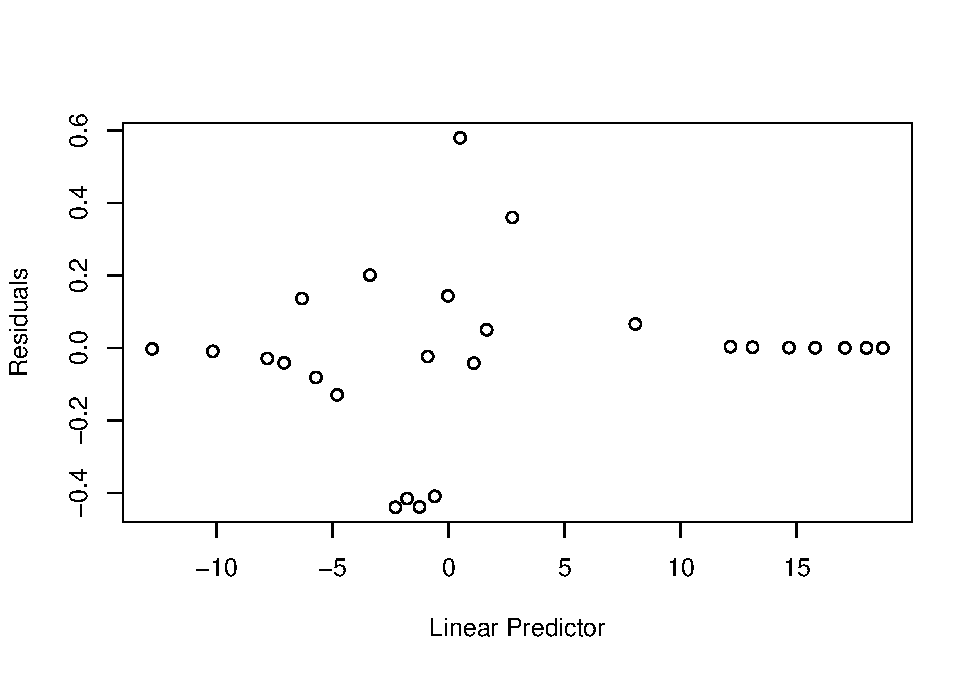
\includegraphics{Data621-Group1-HW4-Final_files/figure-latex/unnamed-chunk-19-1.pdf}

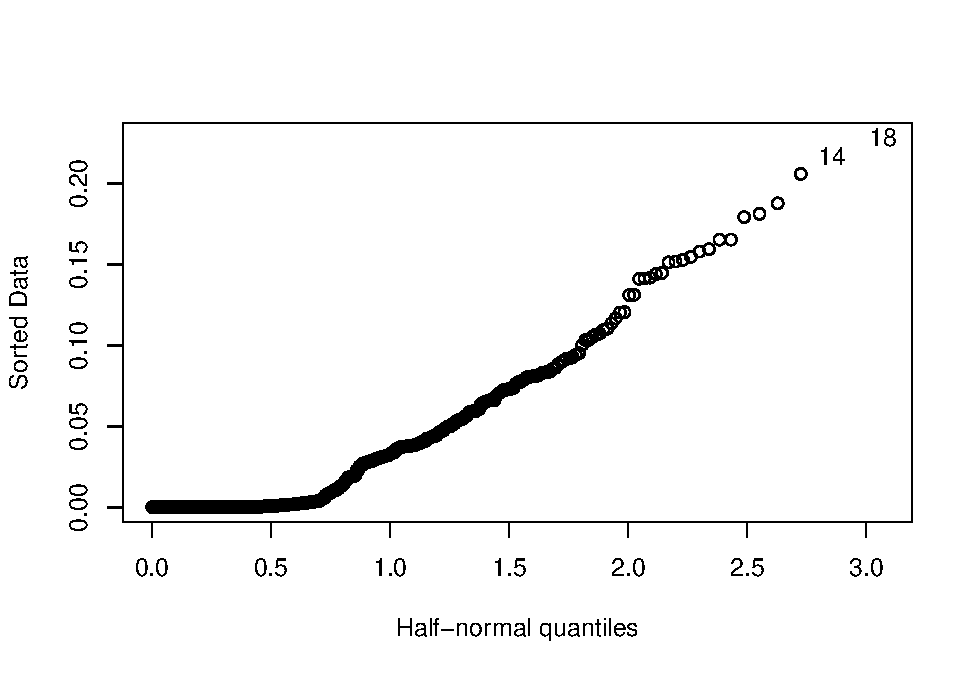
\includegraphics{Data621-Group1-HW4-Final_files/figure-latex/unnamed-chunk-20-1.pdf}

The plot on the right shows that the number of predictors with the
lowest BIC are \texttt{PARENT} , \texttt{HOMEVAL}, \texttt{CAR\_USE},
`CAR\_TYPE', `REVOKED', `MVR\_PTS', `CAR\_AGE' and `URBANICITY'. We will
use those predictors to build the next model

\begin{longtable}[]{@{}ccccc@{}}
\toprule
\begin{minipage}[b]{0.33\columnwidth}\centering
~\strut
\end{minipage} & \begin{minipage}[b]{0.14\columnwidth}\centering
Estimate\strut
\end{minipage} & \begin{minipage}[b]{0.14\columnwidth}\centering
Std. Error\strut
\end{minipage} & \begin{minipage}[b]{0.11\columnwidth}\centering
z value\strut
\end{minipage} & \begin{minipage}[b]{0.13\columnwidth}\centering
Pr(\textgreater\textbar z\textbar)\strut
\end{minipage}\tabularnewline
\midrule
\endhead
\begin{minipage}[t]{0.33\columnwidth}\centering
\textbf{(Intercept)}\strut
\end{minipage} & \begin{minipage}[t]{0.14\columnwidth}\centering
-0.2576\strut
\end{minipage} & \begin{minipage}[t]{0.14\columnwidth}\centering
0.125\strut
\end{minipage} & \begin{minipage}[t]{0.11\columnwidth}\centering
-2.061\strut
\end{minipage} & \begin{minipage}[t]{0.13\columnwidth}\centering
0.03932\strut
\end{minipage}\tabularnewline
\begin{minipage}[t]{0.33\columnwidth}\centering
\textbf{PARENT1Yes}\strut
\end{minipage} & \begin{minipage}[t]{0.14\columnwidth}\centering
0.9691\strut
\end{minipage} & \begin{minipage}[t]{0.14\columnwidth}\centering
0.07619\strut
\end{minipage} & \begin{minipage}[t]{0.11\columnwidth}\centering
12.72\strut
\end{minipage} & \begin{minipage}[t]{0.13\columnwidth}\centering
4.658e-37\strut
\end{minipage}\tabularnewline
\begin{minipage}[t]{0.33\columnwidth}\centering
\textbf{HOME\_VAL}\strut
\end{minipage} & \begin{minipage}[t]{0.14\columnwidth}\centering
-3.481e-06\strut
\end{minipage} & \begin{minipage}[t]{0.14\columnwidth}\centering
4.244e-07\strut
\end{minipage} & \begin{minipage}[t]{0.11\columnwidth}\centering
-8.201\strut
\end{minipage} & \begin{minipage}[t]{0.13\columnwidth}\centering
2.387e-16\strut
\end{minipage}\tabularnewline
\begin{minipage}[t]{0.33\columnwidth}\centering
\textbf{CAR\_USEPrivate}\strut
\end{minipage} & \begin{minipage}[t]{0.14\columnwidth}\centering
-0.8617\strut
\end{minipage} & \begin{minipage}[t]{0.14\columnwidth}\centering
0.06755\strut
\end{minipage} & \begin{minipage}[t]{0.11\columnwidth}\centering
-12.76\strut
\end{minipage} & \begin{minipage}[t]{0.13\columnwidth}\centering
2.888e-37\strut
\end{minipage}\tabularnewline
\begin{minipage}[t]{0.33\columnwidth}\centering
\textbf{CAR\_TYPEPanel Truck}\strut
\end{minipage} & \begin{minipage}[t]{0.14\columnwidth}\centering
0.1519\strut
\end{minipage} & \begin{minipage}[t]{0.14\columnwidth}\centering
0.1238\strut
\end{minipage} & \begin{minipage}[t]{0.11\columnwidth}\centering
1.227\strut
\end{minipage} & \begin{minipage}[t]{0.13\columnwidth}\centering
0.2197\strut
\end{minipage}\tabularnewline
\begin{minipage}[t]{0.33\columnwidth}\centering
\textbf{CAR\_TYPEPickup}\strut
\end{minipage} & \begin{minipage}[t]{0.14\columnwidth}\centering
0.5368\strut
\end{minipage} & \begin{minipage}[t]{0.14\columnwidth}\centering
0.09355\strut
\end{minipage} & \begin{minipage}[t]{0.11\columnwidth}\centering
5.738\strut
\end{minipage} & \begin{minipage}[t]{0.13\columnwidth}\centering
9.6e-09\strut
\end{minipage}\tabularnewline
\begin{minipage}[t]{0.33\columnwidth}\centering
\textbf{CAR\_TYPESports Car}\strut
\end{minipage} & \begin{minipage}[t]{0.14\columnwidth}\centering
1.022\strut
\end{minipage} & \begin{minipage}[t]{0.14\columnwidth}\centering
0.1012\strut
\end{minipage} & \begin{minipage}[t]{0.11\columnwidth}\centering
10.09\strut
\end{minipage} & \begin{minipage}[t]{0.13\columnwidth}\centering
5.897e-24\strut
\end{minipage}\tabularnewline
\begin{minipage}[t]{0.33\columnwidth}\centering
\textbf{CAR\_TYPEVan}\strut
\end{minipage} & \begin{minipage}[t]{0.14\columnwidth}\centering
0.3704\strut
\end{minipage} & \begin{minipage}[t]{0.14\columnwidth}\centering
0.1135\strut
\end{minipage} & \begin{minipage}[t]{0.11\columnwidth}\centering
3.264\strut
\end{minipage} & \begin{minipage}[t]{0.13\columnwidth}\centering
0.001097\strut
\end{minipage}\tabularnewline
\begin{minipage}[t]{0.33\columnwidth}\centering
\textbf{CAR\_TYPEz\_SUV}\strut
\end{minipage} & \begin{minipage}[t]{0.14\columnwidth}\centering
0.7982\strut
\end{minipage} & \begin{minipage}[t]{0.14\columnwidth}\centering
0.08094\strut
\end{minipage} & \begin{minipage}[t]{0.11\columnwidth}\centering
9.862\strut
\end{minipage} & \begin{minipage}[t]{0.13\columnwidth}\centering
6.074e-23\strut
\end{minipage}\tabularnewline
\begin{minipage}[t]{0.33\columnwidth}\centering
\textbf{REVOKEDYes}\strut
\end{minipage} & \begin{minipage}[t]{0.14\columnwidth}\centering
0.78\strut
\end{minipage} & \begin{minipage}[t]{0.14\columnwidth}\centering
0.07661\strut
\end{minipage} & \begin{minipage}[t]{0.11\columnwidth}\centering
10.18\strut
\end{minipage} & \begin{minipage}[t]{0.13\columnwidth}\centering
2.393e-24\strut
\end{minipage}\tabularnewline
\begin{minipage}[t]{0.33\columnwidth}\centering
\textbf{MVR\_PTS}\strut
\end{minipage} & \begin{minipage}[t]{0.14\columnwidth}\centering
0.158\strut
\end{minipage} & \begin{minipage}[t]{0.14\columnwidth}\centering
0.01225\strut
\end{minipage} & \begin{minipage}[t]{0.11\columnwidth}\centering
12.9\strut
\end{minipage} & \begin{minipage}[t]{0.13\columnwidth}\centering
4.487e-38\strut
\end{minipage}\tabularnewline
\begin{minipage}[t]{0.33\columnwidth}\centering
\textbf{URBANICITYz\_Highly Rural/ Rural}\strut
\end{minipage} & \begin{minipage}[t]{0.14\columnwidth}\centering
-2.044\strut
\end{minipage} & \begin{minipage}[t]{0.14\columnwidth}\centering
0.1058\strut
\end{minipage} & \begin{minipage}[t]{0.11\columnwidth}\centering
-19.32\strut
\end{minipage} & \begin{minipage}[t]{0.13\columnwidth}\centering
3.648e-83\strut
\end{minipage}\tabularnewline
\begin{minipage}[t]{0.33\columnwidth}\centering
\textbf{CAR\_AGE}\strut
\end{minipage} & \begin{minipage}[t]{0.14\columnwidth}\centering
-0.036\strut
\end{minipage} & \begin{minipage}[t]{0.14\columnwidth}\centering
0.005397\strut
\end{minipage} & \begin{minipage}[t]{0.11\columnwidth}\centering
-6.669\strut
\end{minipage} & \begin{minipage}[t]{0.13\columnwidth}\centering
2.571e-11\strut
\end{minipage}\tabularnewline
\bottomrule
\end{longtable}

(Dispersion parameter for binomial family taken to be 1 )

\begin{longtable}[]{@{}cc@{}}
\toprule
\endhead
\begin{minipage}[t]{0.27\columnwidth}\centering
Null deviance:\strut
\end{minipage} & \begin{minipage}[t]{0.37\columnwidth}\centering
9418 on 8160 degrees of freedom\strut
\end{minipage}\tabularnewline
\begin{minipage}[t]{0.27\columnwidth}\centering
Residual deviance:\strut
\end{minipage} & \begin{minipage}[t]{0.37\columnwidth}\centering
7827 on 8148 degrees of freedom\strut
\end{minipage}\tabularnewline
\bottomrule
\end{longtable}

\hypertarget{select-model}{%
\subsubsection{Select Model}\label{select-model}}

\hypertarget{compare-model-statistics}{%
\subsubsection{Compare Model
Statistics}\label{compare-model-statistics}}

\hypertarget{model-1---general-model}{%
\subsubsection{Model 1 - General Model}\label{model-1---general-model}}

\textbf{ROC Curve}

The ROC Curve helps measure true positives and true negative. A high AUC
or area under the curve tells us the model is predicting well.

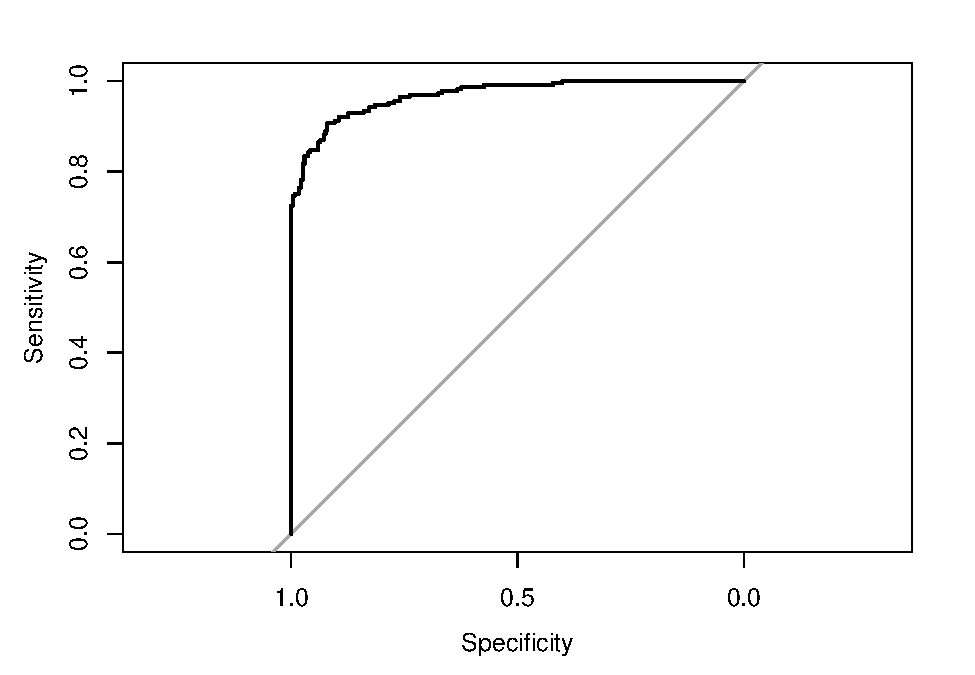
\includegraphics{Data621-Group1-HW4-Final_files/figure-latex/unnamed-chunk-22-1.pdf}

The AUC value of 0.81, tells us this model predicted values are
accurate.

\textbf{Confusion Matrix}

\begin{verbatim}
##          
## targethat    0    1
##         0 5554 1249
##         1  454  904
\end{verbatim}

\textbf{Create a binned diagnostic plot of residuals vs prediction}
There are definite patterns here, which bear investigating.

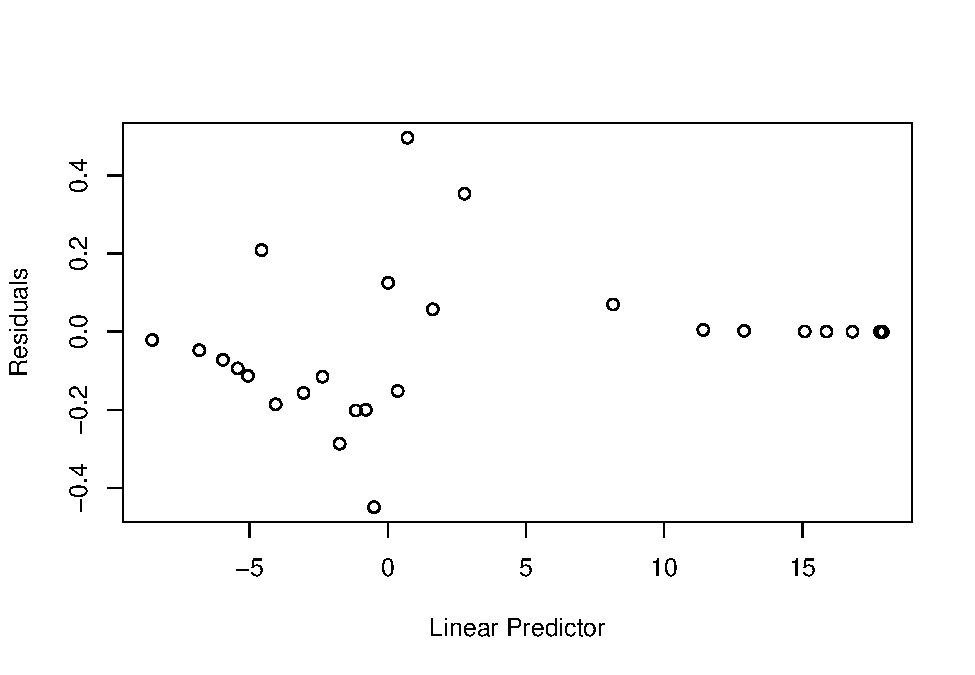
\includegraphics{Data621-Group1-HW4-Final_files/figure-latex/unnamed-chunk-24-1.pdf}

\textbf{Plot leverages.}

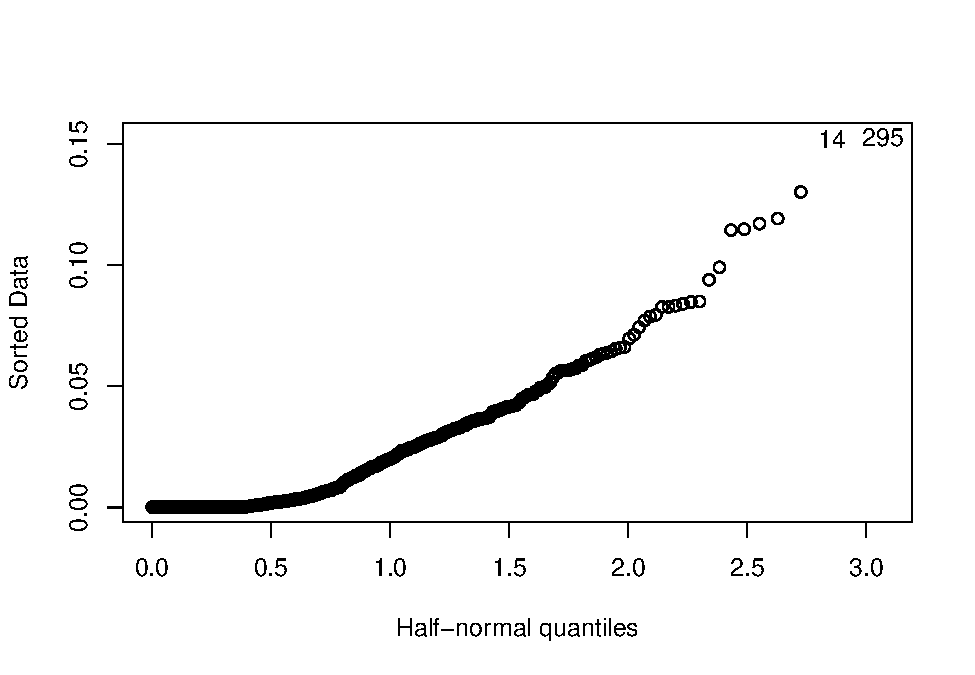
\includegraphics{Data621-Group1-HW4-Final_files/figure-latex/unnamed-chunk-25-1.pdf}

We don't see any strong outliers with the leverage plot. The points
identified (3608,5686) are essentially in the plot of the line formed,
so they are not likely pulling our model in any direction.

\textbf{Plot Goodness of fit}

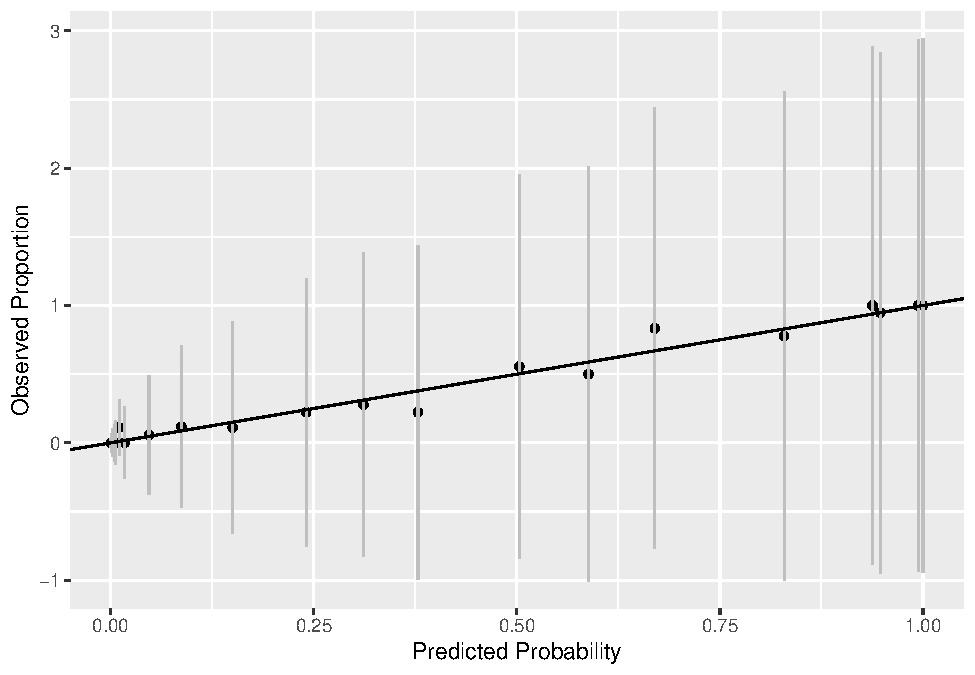
\includegraphics{Data621-Group1-HW4-Final_files/figure-latex/unnamed-chunk-26-1.pdf}

We see that our predictors fall close to the line.

\hypertarget{model-2---reduced-general-model}{%
\subsubsection{Model 2 - Reduced General
Model}\label{model-2---reduced-general-model}}

\textbf{ROC Curve}

The ROC Curve helps measure true positives and true negative. A high AUC
or area under the curve tells us the model is predicting well.

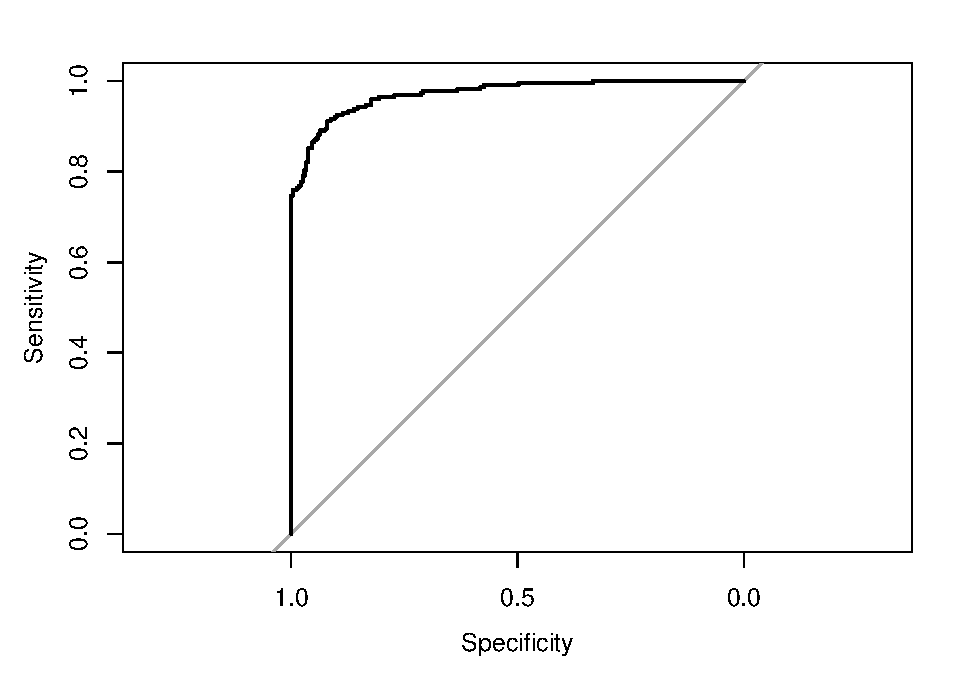
\includegraphics{Data621-Group1-HW4-Final_files/figure-latex/unnamed-chunk-27-1.pdf}

The AUC value of 0.8, tells us this model predicted values are acurate.

\textbf{Confusion Matrix}

\begin{verbatim}
##          
## targethat    0    1
##         0 5559 1296
##         1  449  857
\end{verbatim}

\textbf{Create a binned diagnostic plot of residuals vs prediction}
There are definite patterns here, which bear investigating.

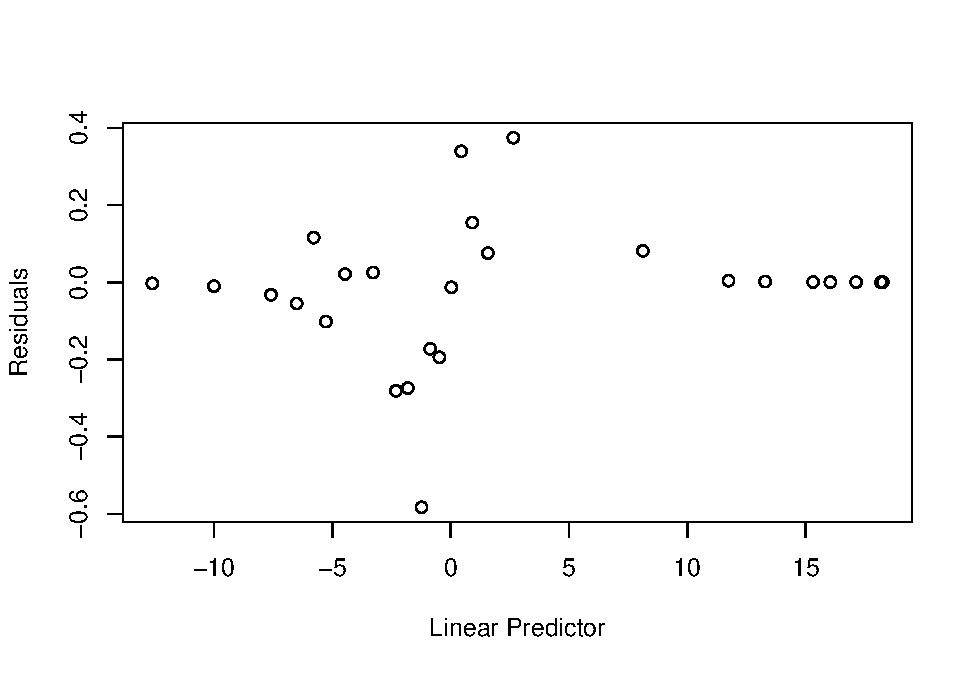
\includegraphics{Data621-Group1-HW4-Final_files/figure-latex/unnamed-chunk-29-1.pdf}

\textbf{Plot leverages.}

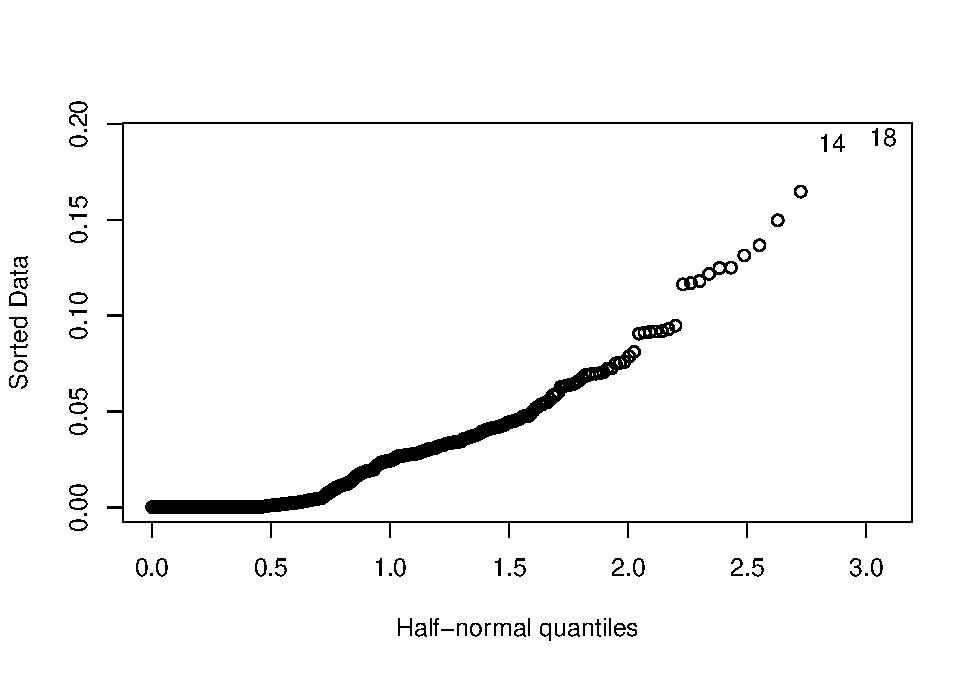
\includegraphics{Data621-Group1-HW4-Final_files/figure-latex/unnamed-chunk-30-1.pdf}

We don't see any strong outliers with the leverage plot. The points
identified (3608,5686) are essentially in the plot of the line formed,
so they are not likely pulling our model in any direction.

\textbf{Plot Goodness of fit}

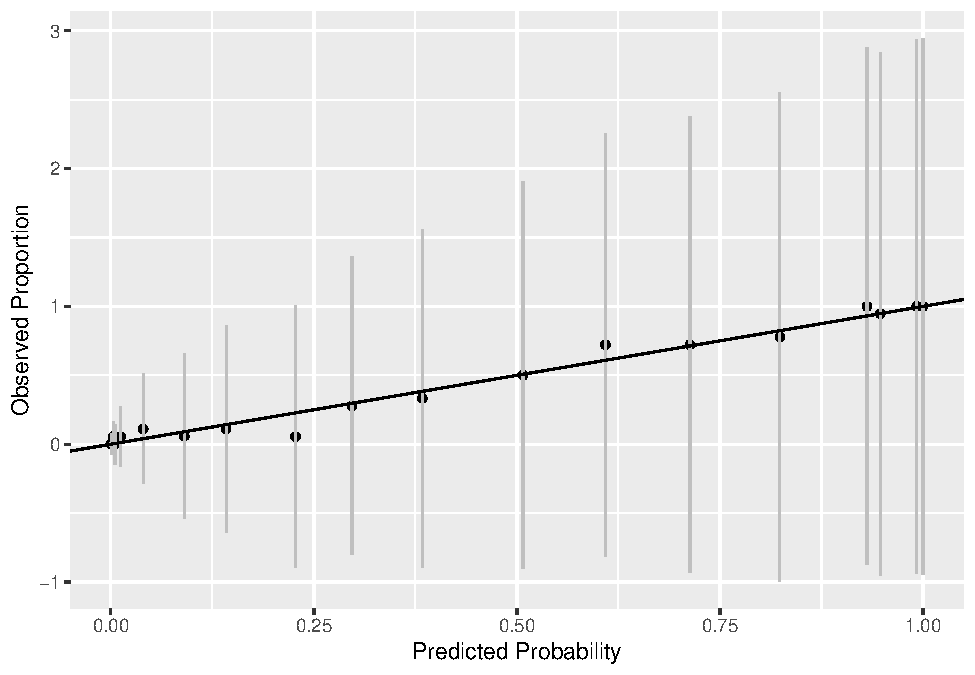
\includegraphics{Data621-Group1-HW4-Final_files/figure-latex/unnamed-chunk-31-1.pdf}

We see that our predictors fall close to the line.

\hypertarget{model-3---srep-aic-model}{%
\subsubsection{Model 3 - Srep AIC
Model}\label{model-3---srep-aic-model}}

\textbf{ROC Curve}

The ROC Curve helps measure true positives and true negative. A high AUC
or area under the curve tells us the model is predicting well.

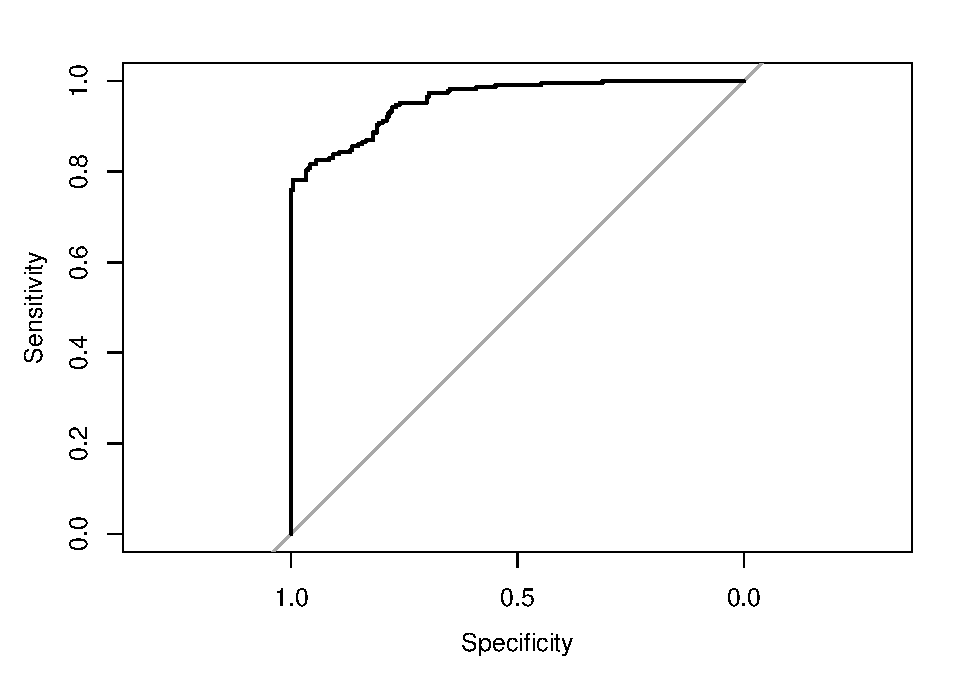
\includegraphics{Data621-Group1-HW4-Final_files/figure-latex/unnamed-chunk-32-1.pdf}

The AUC value of 0.81, tells us this model predicted values are
accurate.

\textbf{Confusion Matrix}

\begin{verbatim}
##          
## targethat    0    1
##         0 5555 1246
##         1  453  907
\end{verbatim}

\textbf{Create a binned diagnostic plot of residuals vs prediction}
There are definite patterns here, which bear investigating.

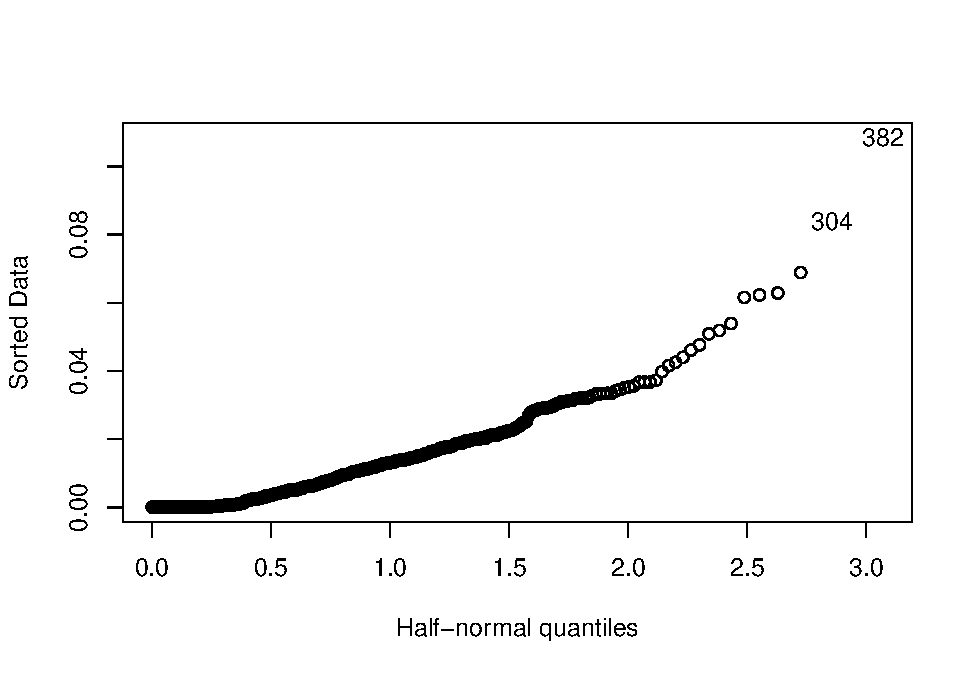
\includegraphics{Data621-Group1-HW4-Final_files/figure-latex/unnamed-chunk-34-1.pdf}

\textbf{Plot leverages.}

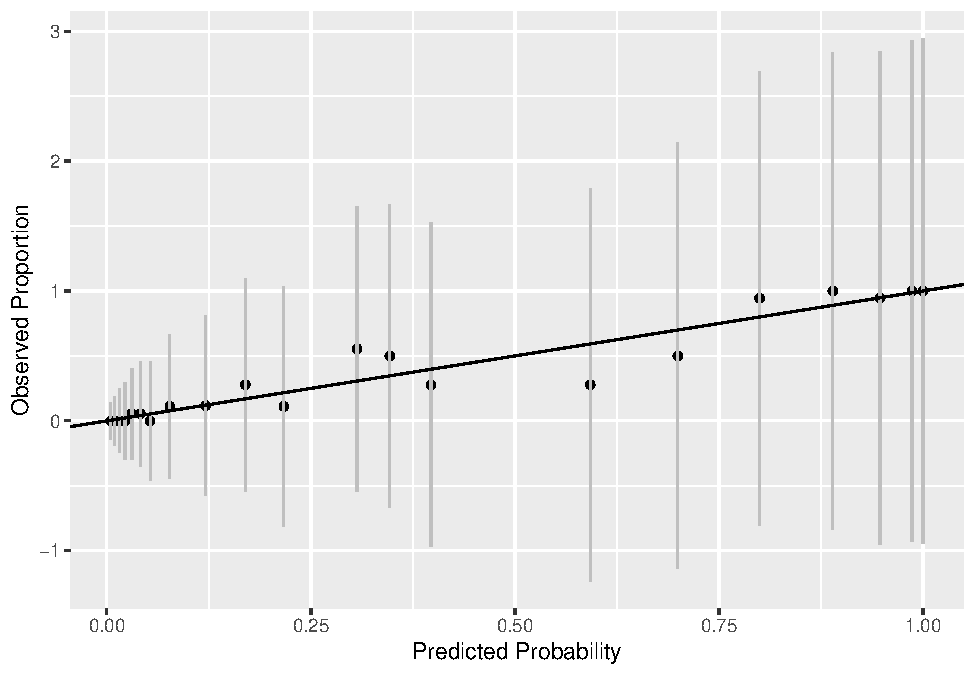
\includegraphics{Data621-Group1-HW4-Final_files/figure-latex/unnamed-chunk-35-1.pdf}

We don't see any strong outliers with the leverage plot. The points
identified (3608,5686) are essentially in the plot of the line formed,
so they are not likely pulling our model in any direction.

\textbf{Plot Goodness of fit}

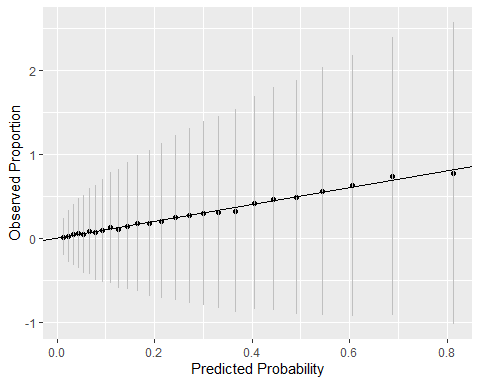
\includegraphics{Data621-Group1-HW4-Final_files/figure-latex/unnamed-chunk-36-1.pdf}

We see that our predictors fall close to the line.

\hypertarget{model-4---srep-bic-model}{%
\subsubsection{Model 4 - Srep BIC
Model}\label{model-4---srep-bic-model}}

\textbf{ROC Curve}

The ROC Curve helps measure true positives and true negative. A high AUC
or area under the curve tells us the model is predicting well.

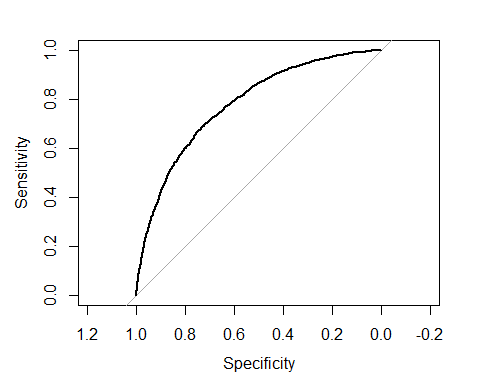
\includegraphics{Data621-Group1-HW4-Final_files/figure-latex/unnamed-chunk-37-1.pdf}

The AUC value of 0.77, tells us this model predicted values are
accurate.

\textbf{Confusion Matrix}

\begin{verbatim}
##          
## targethat    0    1
##         0 5621 1469
##         1  387  684
\end{verbatim}

\textbf{Create a binned diagnostic plot of residuals vs prediction}
There are definite patterns here, which bear investigating.

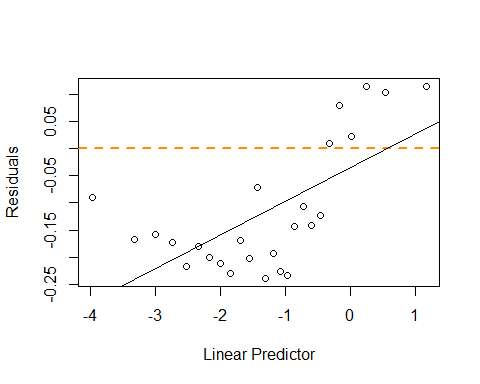
\includegraphics{Data621-Group1-HW4-Final_files/figure-latex/unnamed-chunk-39-1.pdf}

\textbf{Plot leverages.}

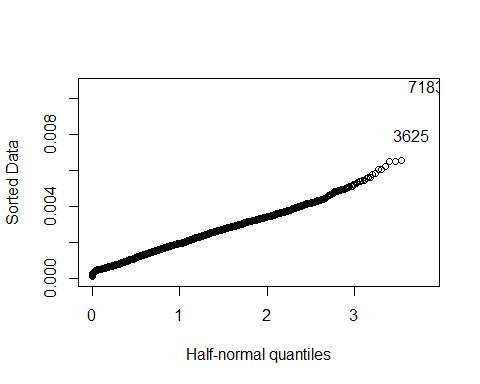
\includegraphics{Data621-Group1-HW4-Final_files/figure-latex/unnamed-chunk-40-1.pdf}

We don't see any strong outliers with the leverage plot. The points
identified (3608,5686) are essentially in the plot of the line formed,
so they are not likely pulling our model in any direction.

\textbf{Plot Goodness of fit}

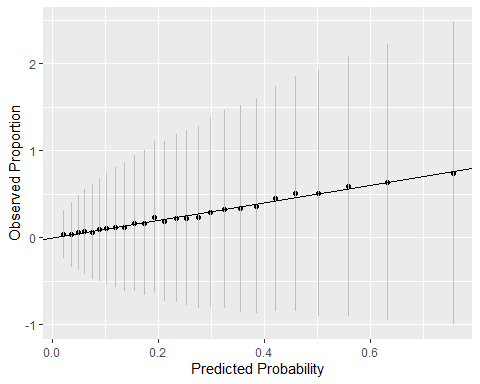
\includegraphics{Data621-Group1-HW4-Final_files/figure-latex/unnamed-chunk-41-1.pdf}

We see that our predictors fall close to the line.

\hypertarget{pick-the-best-regression-model}{%
\subsubsection{Pick the best regression
model}\label{pick-the-best-regression-model}}

\begin{longtable}[]{@{}lllll@{}}
\toprule
Metric & Model 1 & Model 2 & Model 3 & Model 4\tabularnewline
\midrule
\endhead
AIC & 7401.1283155 & 7475.6655813 & 7393.7376519 &
7853.4388014\tabularnewline
BIC & 7660.3918291 & 7650.843631 & 7624.9726775 &
7944.5313873\tabularnewline
\bottomrule
\end{longtable}

With 4 models computed, we select the model with the lowest combination
of AIC and BIC. The the table we can see the model to pick is model 3.

\hypertarget{target_amt-modeling}{%
\subsection{TARGET\_AMT Modeling}\label{target_amt-modeling}}

\textbf{Model 1: all predictors}

Same as with the logistic model before, we start with a model that
includes all predictors

\begin{verbatim}
## 
## Call:
## lm(formula = TARGET_AMT ~ . - TARGET_FLAG, data = InsTrain)
## 
## Residuals:
##    Min     1Q Median     3Q    Max 
##  -5887  -1705   -762    340 103729 
## 
## Coefficients:
##                                   Estimate Std. Error t value Pr(>|t|)    
## (Intercept)                      1.728e+03  4.874e+02   3.545 0.000395 ***
## INDEX                            5.912e-04  1.695e-02   0.035 0.972179    
## KIDSDRIV                         3.143e+02  1.132e+02   2.777 0.005498 ** 
## AGE                              6.023e+00  7.064e+00   0.853 0.393912    
## HOMEKIDS                         8.755e+01  6.557e+01   1.335 0.181875    
## YOJ                             -1.500e+01  1.558e+01  -0.963 0.335611    
## INCOME                          -3.815e-03  2.007e-03  -1.901 0.057371 .  
## PARENT1Yes                       5.761e+02  2.024e+02   2.846 0.004435 ** 
## HOME_VAL                        -5.116e-04  9.887e-04  -0.517 0.604880    
## MSTATUSz_No                      6.231e+02  1.254e+02   4.969 6.86e-07 ***
## SEXz_F                          -3.613e+02  1.838e+02  -1.966 0.049383 *  
## EDUCATIONBachelors              -3.318e+02  2.025e+02  -1.638 0.101447    
## EDUCATIONMasters                -2.261e+02  2.664e+02  -0.849 0.396011    
## EDUCATIONPhD                    -1.204e+01  3.225e+02  -0.037 0.970227    
## EDUCATIONz_High School          -1.187e+02  1.715e+02  -0.692 0.488993    
## JOBDoctor                       -7.980e+02  4.030e+02  -1.980 0.047738 *  
## JOBHome Maker                   -4.945e+01  2.494e+02  -0.198 0.842812    
## JOBLawyer                       -9.920e+01  2.749e+02  -0.361 0.718167    
## JOBManager                      -9.034e+02  2.257e+02  -4.003 6.32e-05 ***
## JOBProfessional                 -2.168e+01  2.122e+02  -0.102 0.918646    
## JOBStudent                      -1.169e+02  2.356e+02  -0.496 0.619786    
## JOBz_Blue Collar                -1.020e+02  1.890e+02  -0.540 0.589356    
## TRAVTIME                         1.207e+01  3.224e+00   3.745 0.000182 ***
## CAR_USEPrivate                  -8.186e+02  1.629e+02  -5.024 5.17e-07 ***
## BLUEBOOK                         1.342e-02  8.609e-03   1.559 0.119094    
## TIF                             -4.835e+01  1.218e+01  -3.968 7.30e-05 ***
## CAR_TYPEPanel Truck              1.558e+02  2.708e+02   0.575 0.565184    
## CAR_TYPEPickup                   3.366e+02  1.695e+02   1.986 0.047021 *  
## CAR_TYPESports Car               1.019e+03  2.179e+02   4.677 2.96e-06 ***
## CAR_TYPEVan                      4.651e+02  2.115e+02   2.199 0.027895 *  
## CAR_TYPEz_SUV                    7.457e+02  1.794e+02   4.157 3.25e-05 ***
## RED_CARyes                      -4.248e+01  1.491e+02  -0.285 0.775670    
## OLDCLAIM                        -1.064e-02  7.439e-03  -1.430 0.152812    
## CLM_FREQ                         1.437e+02  5.505e+01   2.611 0.009048 ** 
## REVOKEDYes                       5.574e+02  1.736e+02   3.212 0.001324 ** 
## MVR_PTS                          1.764e+02  2.592e+01   6.806 1.07e-11 ***
## CAR_AGE                         -2.682e+01  1.280e+01  -2.095 0.036209 *  
## URBANICITYz_Highly Rural/ Rural -1.647e+03  1.391e+02 -11.841  < 2e-16 ***
## ---
## Signif. codes:  0 '***' 0.001 '**' 0.01 '*' 0.05 '.' 0.1 ' ' 1
## 
## Residual standard error: 4546 on 8123 degrees of freedom
## Multiple R-squared:  0.07032,    Adjusted R-squared:  0.06609 
## F-statistic: 16.61 on 37 and 8123 DF,  p-value: < 2.2e-16
\end{verbatim}

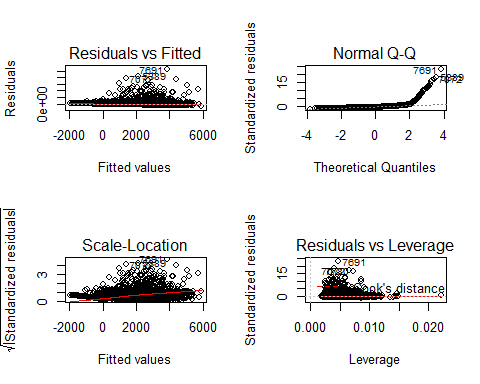
\includegraphics{Data621-Group1-HW4-Final_files/figure-latex/unnamed-chunk-43-1.pdf}

This model shows an adj \(R^2\) as 0.28, and F-statistic of 87.86 with a
small p-value. The result is not a very good model showing a very low
\(R^2\). We also observe several parameters which are not very
significant. We try a second model without these parameters, although we
do not expect it so be much better that this first model.

\textbf{Model 2: Significant predictors}

\begin{verbatim}
## 
## Call:
## lm(formula = TARGET_AMT ~ +AGE + EDUCATION + REVOKED + MVR_PTS + 
##     JOB + YOJ + CLM_FREQ + HOME_VAL + URBANICITY + PARENT1 + 
##     MSTATUS + TRAVTIME + BLUEBOOK, data = InsTrain)
## 
## Residuals:
##    Min     1Q Median     3Q    Max 
##  -5426  -1685   -762    231 104766 
## 
## Coefficients:
##                                   Estimate Std. Error t value Pr(>|t|)    
## (Intercept)                      8.602e+02  3.888e+02   2.212 0.026983 *  
## AGE                              6.055e+00  6.519e+00   0.929 0.353029    
## EDUCATIONBachelors              -3.005e+02  1.843e+02  -1.631 0.102943    
## EDUCATIONMasters                -3.921e+02  2.269e+02  -1.728 0.083988 .  
## EDUCATIONPhD                    -2.272e+02  2.832e+02  -0.802 0.422482    
## EDUCATIONz_High School           4.008e+01  1.647e+02   0.243 0.807697    
## REVOKEDYes                       5.263e+02  1.555e+02   3.384 0.000719 ***
## MVR_PTS                          1.908e+02  2.590e+01   7.369 1.89e-13 ***
## JOBDoctor                       -1.121e+03  3.979e+02  -2.818 0.004850 ** 
## JOBHome Maker                   -9.377e+01  2.451e+02  -0.383 0.702049    
## JOBLawyer                       -4.025e+02  2.689e+02  -1.496 0.134568    
## JOBManager                      -1.009e+03  2.247e+02  -4.492 7.15e-06 ***
## JOBProfessional                 -1.416e+02  2.116e+02  -0.669 0.503241    
## JOBStudent                       2.289e+02  2.285e+02   1.002 0.316516    
## JOBz_Blue Collar                 2.877e+02  1.695e+02   1.697 0.089718 .  
## YOJ                             -6.070e+00  1.481e+01  -0.410 0.681963    
## CLM_FREQ                         1.437e+02  4.896e+01   2.935 0.003346 ** 
## HOME_VAL                        -1.486e-03  8.013e-04  -1.855 0.063629 .  
## URBANICITYz_Highly Rural/ Rural -1.568e+03  1.395e+02 -11.242  < 2e-16 ***
## PARENT1Yes                       8.668e+02  1.802e+02   4.810 1.54e-06 ***
## MSTATUSz_No                      5.094e+02  1.204e+02   4.231 2.35e-05 ***
## TRAVTIME                         1.223e+01  3.238e+00   3.777 0.000160 ***
## BLUEBOOK                         9.345e-03  6.611e-03   1.414 0.157475    
## ---
## Signif. codes:  0 '***' 0.001 '**' 0.01 '*' 0.05 '.' 0.1 ' ' 1
## 
## Residual standard error: 4571 on 8138 degrees of freedom
## Multiple R-squared:  0.05819,    Adjusted R-squared:  0.05565 
## F-statistic: 22.86 on 22 and 8138 DF,  p-value: < 2.2e-16
\end{verbatim}

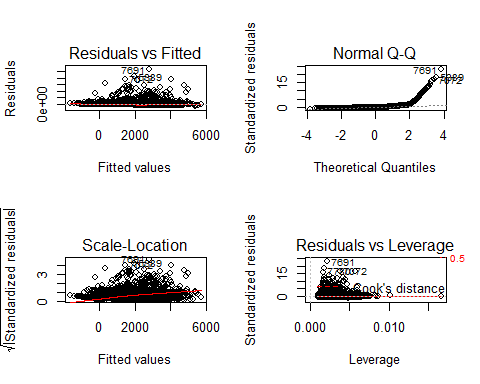
\includegraphics{Data621-Group1-HW4-Final_files/figure-latex/unnamed-chunk-44-1.pdf}

This model shows an adj \(R^2\) as 0.056, and F-statistic of 22.86 with
a small p-value.

Using the reduced predictors, let's now do a stepwise regression:

\textbf{Model 3: Stepwise Regression }

\begin{verbatim}
## Start:  AIC=137577.4
## TARGET_AMT ~ +AGE + EDUCATION + REVOKED + MVR_PTS + JOB + YOJ + 
##     CLM_FREQ + HOME_VAL + URBANICITY + PARENT1 + MSTATUS + TRAVTIME + 
##     BLUEBOOK
## 
##              Df  Sum of Sq        RSS    AIC
## - YOJ         1    3509293 1.7006e+11 137576
## - AGE         1   18026179 1.7007e+11 137576
## - EDUCATION   4  154037045 1.7021e+11 137577
## <none>                     1.7006e+11 137577
## - BLUEBOOK    1   41765295 1.7010e+11 137577
## - HOME_VAL    1   71907597 1.7013e+11 137579
## - CLM_FREQ    1  179988338 1.7024e+11 137584
## - REVOKED     1  239252115 1.7030e+11 137587
## - TRAVTIME    1  298134916 1.7035e+11 137590
## - MSTATUS     1  374117944 1.7043e+11 137593
## - PARENT1     1  483407044 1.7054e+11 137599
## - JOB         7 1186770595 1.7124e+11 137620
## - MVR_PTS     1 1134624808 1.7119e+11 137630
## - URBANICITY  1 2640997262 1.7270e+11 137701
## 
## Step:  AIC=137575.6
## TARGET_AMT ~ AGE + EDUCATION + REVOKED + MVR_PTS + JOB + CLM_FREQ + 
##     HOME_VAL + URBANICITY + PARENT1 + MSTATUS + TRAVTIME + BLUEBOOK
## 
##              Df  Sum of Sq        RSS    AIC
## - AGE         1   16550382 1.7008e+11 137574
## - EDUCATION   4  153627889 1.7021e+11 137575
## - BLUEBOOK    1   41120143 1.7010e+11 137576
## <none>                     1.7006e+11 137576
## - HOME_VAL    1   72557883 1.7013e+11 137577
## - CLM_FREQ    1  180284088 1.7024e+11 137582
## - REVOKED     1  239230021 1.7030e+11 137585
## - TRAVTIME    1  297722480 1.7036e+11 137588
## - MSTATUS     1  398431642 1.7046e+11 137593
## - PARENT1     1  479908120 1.7054e+11 137597
## - JOB         7 1194946049 1.7125e+11 137619
## - MVR_PTS     1 1138469809 1.7120e+11 137628
## - URBANICITY  1 2638652491 1.7270e+11 137699
## 
## Step:  AIC=137574.4
## TARGET_AMT ~ EDUCATION + REVOKED + MVR_PTS + JOB + CLM_FREQ + 
##     HOME_VAL + URBANICITY + PARENT1 + MSTATUS + TRAVTIME + BLUEBOOK
## 
##              Df  Sum of Sq        RSS    AIC
## - EDUCATION   4  152052323 1.7023e+11 137574
## <none>                     1.7008e+11 137574
## - BLUEBOOK    1   45832097 1.7012e+11 137575
## - HOME_VAL    1   68168845 1.7014e+11 137576
## - CLM_FREQ    1  183048294 1.7026e+11 137581
## - REVOKED     1  237194155 1.7031e+11 137584
## - TRAVTIME    1  299955129 1.7038e+11 137587
## - MSTATUS     1  407190173 1.7048e+11 137592
## - PARENT1     1  468406609 1.7054e+11 137595
## - JOB         7 1179606130 1.7126e+11 137617
## - MVR_PTS     1 1129124172 1.7121e+11 137626
## - URBANICITY  1 2630482199 1.7271e+11 137698
## 
## Step:  AIC=137573.6
## TARGET_AMT ~ REVOKED + MVR_PTS + JOB + CLM_FREQ + HOME_VAL + 
##     URBANICITY + PARENT1 + MSTATUS + TRAVTIME + BLUEBOOK
## 
##              Df  Sum of Sq        RSS    AIC
## - BLUEBOOK    1   32875890 1.7026e+11 137573
## <none>                     1.7023e+11 137574
## - HOME_VAL    1  119051672 1.7035e+11 137577
## - CLM_FREQ    1  181086747 1.7041e+11 137580
## - REVOKED     1  241380620 1.7047e+11 137583
## - TRAVTIME    1  292522009 1.7052e+11 137586
## - MSTATUS     1  387615210 1.7062e+11 137590
## - PARENT1     1  485655803 1.7071e+11 137595
## - MVR_PTS     1 1137578413 1.7137e+11 137626
## - JOB         7 1790035008 1.7202e+11 137645
## - URBANICITY  1 2578301343 1.7281e+11 137694
## 
## Step:  AIC=137573.2
## TARGET_AMT ~ REVOKED + MVR_PTS + JOB + CLM_FREQ + HOME_VAL + 
##     URBANICITY + PARENT1 + MSTATUS + TRAVTIME
## 
##              Df  Sum of Sq        RSS    AIC
## <none>                     1.7026e+11 137573
## - HOME_VAL    1   95590131 1.7036e+11 137576
## - CLM_FREQ    1  178112068 1.7044e+11 137580
## - REVOKED     1  237961372 1.7050e+11 137583
## - TRAVTIME    1  293078406 1.7055e+11 137585
## - MSTATUS     1  393037079 1.7065e+11 137590
## - PARENT1     1  476844375 1.7074e+11 137594
## - MVR_PTS     1 1131360137 1.7139e+11 137625
## - JOB         7 1781608903 1.7204e+11 137644
## - URBANICITY  1 2593045561 1.7285e+11 137695
\end{verbatim}

\begin{verbatim}
## 
## Call:
## lm(formula = TARGET_AMT ~ REVOKED + MVR_PTS + JOB + CLM_FREQ + 
##     HOME_VAL + URBANICITY + PARENT1 + MSTATUS + TRAVTIME, data = InsTrain)
## 
## Residuals:
##    Min     1Q Median     3Q    Max 
##  -5553  -1689   -758    210 104765 
## 
## Coefficients:
##                                   Estimate Std. Error t value Pr(>|t|)    
## (Intercept)                      1.158e+03  2.268e+02   5.106 3.36e-07 ***
## REVOKEDYes                       5.246e+02  1.555e+02   3.374 0.000744 ***
## MVR_PTS                          1.903e+02  2.587e+01   7.357 2.07e-13 ***
## JOBDoctor                       -1.202e+03  3.378e+02  -3.559 0.000374 ***
## JOBHome Maker                   -1.700e+02  2.227e+02  -0.763 0.445339    
## JOBLawyer                       -6.757e+02  2.156e+02  -3.135 0.001727 ** 
## JOBManager                      -1.170e+03  2.081e+02  -5.621 1.97e-08 ***
## JOBProfessional                 -2.957e+02  1.951e+02  -1.516 0.129666    
## JOBStudent                       2.284e+02  2.154e+02   1.060 0.289019    
## JOBz_Blue Collar                 2.416e+02  1.656e+02   1.459 0.144644    
## CLM_FREQ                         1.428e+02  4.893e+01   2.919 0.003521 ** 
## HOME_VAL                        -1.569e-03  7.339e-04  -2.138 0.032512 *  
## URBANICITYz_Highly Rural/ Rural -1.548e+03  1.390e+02 -11.138  < 2e-16 ***
## PARENT1Yes                       8.206e+02  1.718e+02   4.776 1.82e-06 ***
## MSTATUSz_No                      5.129e+02  1.183e+02   4.336 1.47e-05 ***
## TRAVTIME                         1.212e+01  3.237e+00   3.744 0.000182 ***
## ---
## Signif. codes:  0 '***' 0.001 '**' 0.01 '*' 0.05 '.' 0.1 ' ' 1
## 
## Residual standard error: 4572 on 8145 degrees of freedom
## Multiple R-squared:  0.05706,    Adjusted R-squared:  0.05532 
## F-statistic: 32.86 on 15 and 8145 DF,  p-value: < 2.2e-16
\end{verbatim}

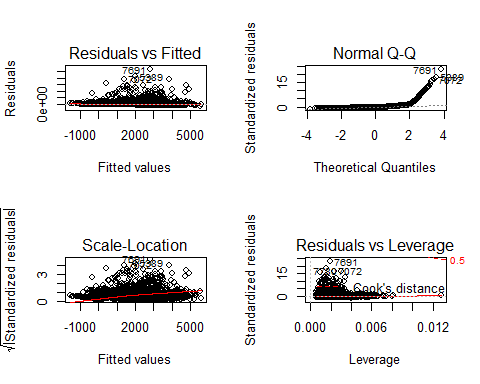
\includegraphics{Data621-Group1-HW4-Final_files/figure-latex/unnamed-chunk-45-1.pdf}

This model shows an adj \(R^2\) as 0.055, and F-statistic of 32.86 with
a small p-value. As expected this model isn't any better than the first
one. It is simpler, but its performance is basically the same. What we
do notice, and very visible in the Q-Q plot, is that these seem to be a
high number of data points distance from the normal. This suggest a
different kind of model.

\textbf{Model 4: Weighted coefficients}

We build a Hubber weigthed model to account for the distant points
observed in the previous models.

\begin{verbatim}
## 
## Call: rlm(formula = TARGET_AMT ~ . - TARGET_FLAG, data = InsTrain, 
##     maxit = 40)
## Residuals:
##      Min       1Q   Median       3Q      Max 
##  -2047.0   -492.2   -133.3    503.8 106540.0 
## 
## Coefficients:
##                                 Value     Std. Error t value  
## (Intercept)                      676.8268   94.2063     7.1845
## INDEX                             -0.0001    0.0033    -0.0153
## KIDSDRIV                         139.0172   21.8765     6.3546
## AGE                               -0.0529    1.3652    -0.0387
## HOMEKIDS                           8.7242   12.6732     0.6884
## YOJ                               -8.8665    3.0102    -2.9455
## INCOME                            -0.0009    0.0004    -2.2019
## PARENT1Yes                       274.0114   39.1159     7.0051
## HOME_VAL                           0.0001    0.0002     0.7054
## MSTATUSz_No                      169.7873   24.2341     7.0061
## SEXz_F                           -26.5180   35.5257    -0.7464
## EDUCATIONBachelors              -168.5739   39.1421    -4.3067
## EDUCATIONMasters                -173.2367   51.4839    -3.3649
## EDUCATIONPhD                    -190.1227   62.3261    -3.0505
## EDUCATIONz_High School            11.8464   33.1433     0.3574
## JOBDoctor                       -146.8373   77.8923    -1.8851
## JOBHome Maker                      7.0630   48.1974     0.1465
## JOBLawyer                        -82.4219   53.1218    -1.5516
## JOBManager                      -281.5451   43.6208    -6.4544
## JOBProfessional                  -88.4633   41.0165    -2.1568
## JOBStudent                        -9.3306   45.5270    -0.2049
## JOBz_Blue Collar                 -83.1141   36.5182    -2.2760
## TRAVTIME                           3.9424    0.6230     6.3281
## CAR_USEPrivate                  -300.8995   31.4928    -9.5546
## BLUEBOOK                          -0.0052    0.0017    -3.1514
## TIF                              -15.6168    2.3549    -6.6317
## CAR_TYPEPanel Truck               30.2631   52.3424     0.5782
## CAR_TYPEPickup                   130.2403   32.7521     3.9765
## CAR_TYPESports Car               278.0083   42.1038     6.6029
## CAR_TYPEVan                       93.9587   40.8706     2.2989
## CAR_TYPEz_SUV                    199.0489   34.6674     5.7417
## RED_CARyes                        -2.1157   28.8124    -0.0734
## OLDCLAIM                          -0.0043    0.0014    -2.9666
## CLM_FREQ                          55.3530   10.6402     5.2023
## REVOKEDYes                       387.5239   33.5434    11.5529
## MVR_PTS                           63.4666    5.0093    12.6697
## CAR_AGE                           -0.1901    2.4742    -0.0768
## URBANICITYz_Highly Rural/ Rural -550.0751   26.8871   -20.4587
## 
## Residual standard error: 733.5 on 8123 degrees of freedom
\end{verbatim}

\includegraphics{Data621-Group1-HW4-Final_files/figure-latex/unnamed-chunk-46-1.pdf}

The models doesn't seem to help with weigthed coefficients, we stil see
the effects of several datapoints in the data.

\hypertarget{pick-the-best-regression-model-1}{%
\subsubsection{Pick the best regression
model}\label{pick-the-best-regression-model-1}}

\begin{longtable}[]{@{}lllll@{}}
\toprule
Metric & Model 1 & Model 2 & Model 3 & Model 4\tabularnewline
\midrule
\endhead
AIC & \ensuremath{1.606635\times 10^{5}} &
\ensuremath{1.607393\times 10^{5}} & \ensuremath{1.6073514\times 10^{5}}
& \ensuremath{1.6133706\times 10^{5}}\tabularnewline
BIC & \ensuremath{1.6093677\times 10^{5}} &
\ensuremath{1.6090748\times 10^{5}} &
\ensuremath{1.6085426\times 10^{5}} &
\ensuremath{1.6161034\times 10^{5}}\tabularnewline
\bottomrule
\end{longtable}

With 4 models computed, we select the model with the lowest combination
of AIC and BIC. The model to pick is model 3.

\hypertarget{conclusion}{%
\subsection{Conclusion}\label{conclusion}}

For both the logistic regression and linear regressions we picked model
3. Results for the logistic regression were rather good, but the linear
regression doesn't seem to be a good model, even when using weigthed
coefficients.

\begin{verbatim}
## Observations: 2,141
## Variables: 4
## $ INCOME   <fct> "$52,881", "$50,815", "$43,486", "$21,204", "$87,460"...
## $ HOME_VAL <fct> "$0", "$0", "$0", "$0", "$0", "$207,519", "$182,739",...
## $ BLUEBOOK <fct> "$21,970", "$18,930", "$5,900", "$9,230", "$15,420", ...
## $ OLDCLAIM <fct> "$0", "$3,295", "$0", "$0", "$44,857", "$2,119", "$0"...
## Observations: 2,141
## Variables: 4
## $ INCOME   <int> 52881, 50815, 43486, 21204, 87460, NA, 37940, 33212, ...
## $ HOME_VAL <int> 0, 0, 0, 0, 0, 207519, 182739, 158432, 344195, 0, 176...
## $ BLUEBOOK <int> 21970, 18930, 5900, 9230, 15420, 25660, 11290, 24000,...
## $ OLDCLAIM <int> 0, 3295, 0, 0, 44857, 2119, 0, 0, 0, 0, 0, 0, 0, 2045...
\end{verbatim}

\hypertarget{appendix}{%
\section{APPENDIX}\label{appendix}}

\textbf{Code used in analysis}

knitr::opts\_chunk\$set(echo = FALSE, warning = FALSE) require(knitr)
library(ggplot2) library(tidyr) library(MASS) library(psych)
library(kableExtra) library(dplyr) library(faraway) library(gridExtra)
library(reshape2) library(leaps) library(pROC) library(caret)
library(naniar) library(pander) library(pROC)

Get the data. Added na.strings to add na for records that have a blank
value

InsTrain \textless-
read.csv(``insurance\_training\_data.csv'',na.strings="``,header=TRUE)
InsEval \textless-
read.csv(''insurance-evaluation-data.csv``,na.strings=''",header=TRUE)
InsEval \textless- subset(InsEval, select=-c(TARGET\_FLAG,TARGET\_AMT))

InsEval \textless-
read.csv(``insurance-evaluation-data.csv'',na.strings="",header=TRUE)

OVERVIEW

In this homework assignment, you will explore, analyze and model a data
set containing approximately 8000 records representing a customer at an
auto insurance company. Each record has two response variables. The
first response variable, TARGET\_FLAG, is a 1 or a 0. A ``1'' means that
the person was in a car crash. A zero means that the person was not in a
car crash. The second response variable is TARGET\_AMT. This value is
zero if the person did not crash their car. But if they did crash their
car, this number will be a value greater than zero representing the cost
of the crash.

Objective:

Your objective is to build multiple linear regression and binary
logistic regression models on the training data to predict the
probability that a person will crash their car and also the amount of
money it will cost if the person does crash their car.

DATA EXPLORATION

Data Summary

ins1 \textless- describe(InsTrain, na.rm = F)
ins1\(na_count <- sapply(InsTrain, function(y) sum(length(which(is.na(y))))) ins1\)na\_count\_perc
\textless- sapply(InsTrain, function(x)
round(sum(is.na(x))/nrow(InsTrain)*100,1))

colsTrain\textless-ncol(InsTrain) colsEval\textless-ncol(InsEval)
missingCol\textless-colnames(InsTrain){[}!(colnames(InsTrain) \%in\%
colnames(InsEval)){]}

The dataset consists of two data files: training and evaluation. The
training dataset contains 26 columns, while the evaluation dataset
contains 26. The evaluation dataset is missing columns which represent
our response variables, respectively whether the person was in a car
crash and the cost of the car crash if the person was in an accident. We
will start by exploring the training data set since it will be the one
used to generate the models.

The columns in the data set are:\\
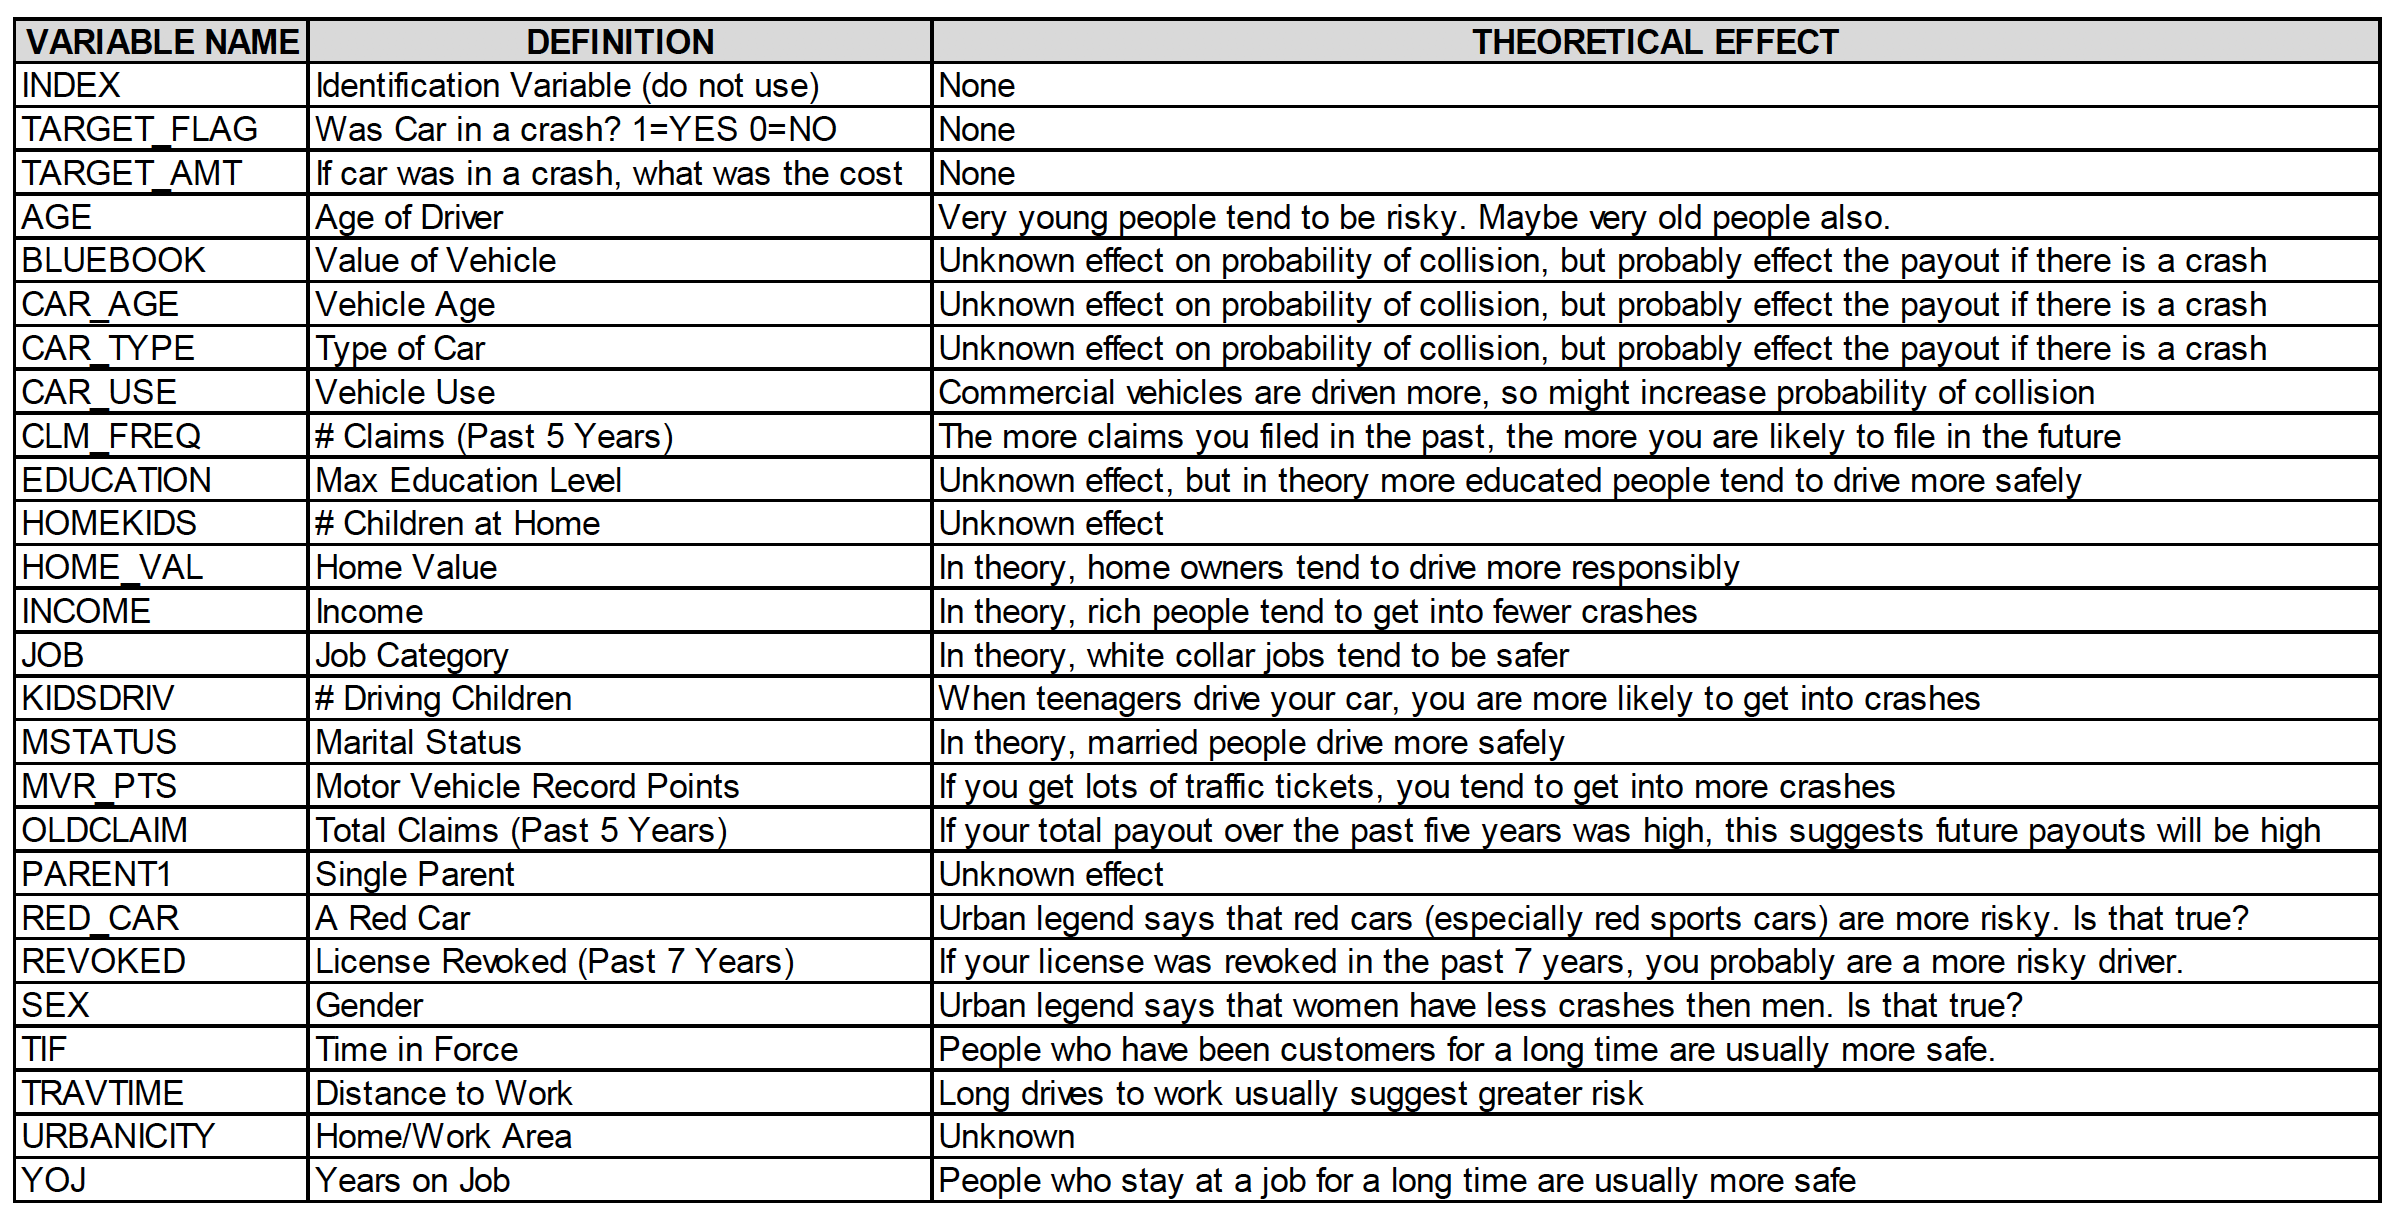
\includegraphics{dataTable.png}

Missing Data

An important aspect of any dataset is to determine how much, if any,
data is missing. We look at all the variables to see which if any have
missing data. We look at the basic descriptive statistics as well as the
missing data and percentages.

We start by looking at the dataset as a whole and determine how many
complete rows, that is rows with data for all predictors, do we have.

cc\textless-summary(complete.cases(InsTrain))
cInsTrain\textless-subset(InsTrain, complete.cases(InsTrain)) cc

With these results, if we remove all rows with incomplete rows, there
will be a total of 6045 rows out of 8161 .If we eliminate all
non-complete rows and keep only rows with data for all the predictors in
the dataset, our new dataset will results in 74\% of the total dataset.
We create a subset of data with complete cases only to use later in our
analysis.

glimpse(cInsTrain)

But we can also look at what specific predictors are missing in our
dataset. If we do this we can see how there is much more data available,
as we find only 5 predictors with missing data. Data missing for these
predictors also only accounts for less than 7\% of the respective
predictors total.

vis\_miss(InsTrain)

We look closer at the missing data and look at the intersection of
predictors with missing data. We find that the bulk of the missing data
is for predictors with no intersection with other missing predictor
data.

gg\_miss\_upset(InsTrain)

Having this detail in missing data might be of importance when looking
at models. In the next Data Preparation section we will handle these
missing cases and build a data set with data for all predictors in all
rows.

Data Exploration

Using TARGET\_FLAG as response variables we confirm when TARGET\_FLAG is
1 TARGET\_AMOUNT \textgreater0 and when TARGET\_FLAG is 0 when
TARGET\_AMOUNT = 0

nrow(subset(InsTrain,TARGET\_FLAG == 0))
nrow(subset(InsTrain,TARGET\_AMT == 0))
nrow(subset(InsTrain,TARGET\_FLAG \textgreater{} 0))
nrow(subset(InsTrain,TARGET\_AMT \textgreater{} 0))

A glimpse of the data shows that the following columns should be
integers and not Factors:

\begin{itemize}
\tightlist
\item
  INCOME
\item
  HOME\_VAL
\item
  BLUEBOOK
\item
  OLDCLAIM
\end{itemize}

We display and view data with all cases and only complete cases

cat(colnames(InsTrain{[} sapply(InsTrain, is.factor){]}), ``\n\n'')
glimpse(InsTrain)

We use Sapply function to review which columns have NA Values. It
display columns and percent of values that are missing.

sapply(InsTrain, function(x) round(sum(is.na(x))/nrow(InsTrain)*100,1))

Data Preparation

As revealed earlier there were a list of columns that we factors that
should be integers. We start by converting the columns to numeric.

c\textless-c(`INCOME',`HOME\_VAL',`BLUEBOOK',`OLDCLAIM') if(c \%in\%
colnames(InsTrain))\{

glimpse(InsTrain{[},(c){]}) InsTrain{[},c{]} \textless-
sapply(InsTrain{[},(c){]}, function(x)
as.integer(gsub(`{[}\$,{]}','',as.character(x))))

glimpse(InsTrain{[},(c){]})

\} else \{

cat(``Please review your selection of columns:'', c)

\}

Both boxplot and summary stats with the square root transform of
Home\_val and Income to confirm we can use median or mean values to
replace NA values if we chose.

InsTrain\(INCOME <- na_if(InsTrain\)INCOME, 0)
InsTrain\(HOME_VAL <- na_if(InsTrain\)HOME\_VAL, 0) r \textless-
colnames(InsTrain{[} sapply(InsTrain, function(x) return(anyNA(x) \&\&
is.integer(x))){]}) boxplot(InsTrain{[},r{]},names = r,las = 2,col =
c(``orange'',``red'', ``blue'', ``yellow'', ``brown'', ``green''))
describe(subset(InsTrain, select =r))

We next replace all NA values with mean values for cases that are
missing values and rerun sapply function to confirm there are no longer
any missing values.

sapply(InsTrain, function(x) round(sum(is.na(x))/nrow(InsTrain)*100,1))

InsTrain{[},r{]} \textless- replace\_na(InsTrain{[},r{]},
as.list(colMeans(InsTrain{[},r{]}, na.rm = TRUE))) Jobs \textless-
summary(InsTrain\(JOB) print(Jobs) JobsMode <- Jobs[which.max(Jobs)] ifelse(JobsMode[[1]] / nrow(InsTrain) > 2.5*(Jobs["NA's"][[1]] / nrow(InsTrain)),  InsTrain\)JOB
\textless-
replace\_na(InsTrain\(JOB, names(JobsMode)),  na.omit(InsTrain)  ) summary(InsTrain\)JOB)

vis\_miss(InsTrain) describe(subset(InsTrain, select =r))

We have this way derived a dataset with no missing values. We can use
this set of data for our modeling design. We chose to work with this
data as opposed to the first ``complete'' set in which rows with missing
data were eliminated.

Build Model

Modeling design will be divided in two phases. First we will design a
model to predict if the person is in a car crash, that is predict
TARGET\_FLAG. In a second phase, we will predict TARGET\_AMT, the cost
of the crash.

TARGET\_FLAG Modeling

This response variable being binary, o or 1, we will be looking at
logistic regression models to find a good fit. We will start with a
naive model with all the predictors included as a baseline. First
approach will be to simply the model by reducing the predictors used. We
will look at several model metrics such as AIC, BIC. We will also
include confusion tables and ROC plot to better understand each model.

\textbf{Model 1: all predictors}

We start out with a straightforward logit logistical regression with all
predictors included. As a note, we need to make sure we do not include
the TARGET\_AMT responce variable in our model as a predictor.

m1\textless-glm(TARGET\_FLAG\textasciitilde.-INDEX-TARGET\_AMT,data=InsTrain,family=``binomial''(link=``logit''))
summary(m1)

From the model's summary itself we see that there are several predictors
which are not statistically relevant, which suggestes a simpler model
should be possible. We build a second model without these the
non-significant predictors.

\textbf{Model 2: reduced predictors}

m2\textless-glm(TARGET\_FLAG\textasciitilde.-INDEX-TARGET\_AMT-AGE-INCOME-JOB-BLUEBOOK-CAR\_AGE-RED\_CAR,data=InsTrain,family=``binomial''(link=``logit''))
summary(m2)

The new model has a slightly higher AIC which would tells us the first
model is slightly less complex.

AIC Step Method Model 3

Another way of selecting which predictors to use in the model is by
calculating the AIC of the model. This metric is similar to the adjusted
R-square of a model in that it penalizes models with more predictors
over simpler model with few predictors. We use Stepwise function in r to
find the lowest AIC with different predictors.

m3 \textless- step(m1) summary(m3)

This reduces the predictors used to 25 from 30. The AIC is reduced from
7401.13 (our original general model) to 7393.7, just slightly and but we
benefit by having a simpler model less prone to overfitting.

Also, the predictors in the model now are all signficant (under 0.05 pr
level) and all but one under .02 or very significant. Which is much
improved over the first model.

BIC Method Model 4

To determine the number of predictors and which predictors to be used we
will use the Bayesian Information Criterion (BIC).

InsTrainM4\textless-InsTrain{[} , !(names(InsTrain) \%in\%
c(`INDEX',`TARGET\_AMT')){]} regfit.full \textless-
regsubsets(factor(TARGET\_FLAG) \textasciitilde{} ., data=InsTrainM4)
par(mfrow = c(1,2)) reg.summary \textless- summary(regfit.full)
plot(reg.summary\(bic, xlab="Number of Predictors", ylab="BIC", type="l", main="Subset Selection Using BIC") BIC_num <- which.min(reg.summary\)bic)
points(BIC\_num, reg.summary\$bic{[}BIC\_num{]}, col=``red'', cex=2,
pch=20)

plot(regfit.full, scale=``bic'', main=``Predictors vs.~BIC'', asp = 10)

The plot on the right shows that the number of predictors with the
lowest BIC are \texttt{PARENT} , \texttt{HOMEVAL}, \texttt{CAR\_USE},
`CAR\_TYPE', `REVOKED', `MVR\_PTS', `CAR\_AGE' and `URBANICITY'. We will
use those predictors to build the next model

m4 \textless- glm(TARGET\_FLAG \textasciitilde{} PARENT1 + HOME\_VAL +
CAR\_USE + CAR\_TYPE + REVOKED + MVR\_PTS + URBANICITY + CAR\_AGE,
family=binomial, data = InsTrain)
InsTrain\(predicted_m3<- predict(m4, InsTrain, type='response') InsTrain\)target\_m4\(target <- ifelse(InsTrain\)predicted\_m4\textgreater0.5,
1, 0) pander::pander(summary(m4))

Select Model

Model 1 - General Model

\textbf{ROC Curve}

The ROC Curve helps measure true positives and true negative. A high AUC
or area under the curve tells us the model is predicting well.

targethat\textless-predict(m1,type=``response'')
g\textless-roc(TARGET\_FLAG\textasciitilde targethat,data=InsTrain)
plot(g)

The AUC value of 0.77, tells us this model predicted values are acurate.

\textbf{Confusion Matrix}

targethat{[}targethat\textless0.5{]}\textless-0
targethat{[}targethat\textgreater=0.5{]}\textless-1
table(targethat,InsTrain\$TARGET\_FLAG)

\textbf{Create a binned diagnostic plot of residuals vs prediction}
There are definite patterns here, which bear investigating.

InsMut \textless- mutate(InsTrain, Residuals = residuals(m1), linPred =
predict(m1)) grpIns \textless- group\_by(InsMut, cut(linPred,
breaks=unique(quantile(linPred, (0:25/26))))) diagIns \textless-
summarise(grpIns, Residuals = mean(Residuals), linPred = mean(linPred))
plot(Residuals \textasciitilde{} linPred, data = diagIns, xlab=``Linear
Predictor'') abline(h = 0, lty = 2, col = ``darkorange'', lwd = 2)

\textbf{Plot leverages.}

halfnorm(hatvalues(m1))

We don't see any strong outliers with the leverage plot. The points
identified (3608,5686) are essentially in the plot of the line formed,
so they are not likely pulling our model in any direction.

\textbf{Plot Goodness of fit}

linPred \textless- predict(m1) InsMut \textless- mutate(InsTrain,
predProb = predict(m1, type = ``response'')) grpIns \textless-
group\_by(InsMut, cut(linPred, breaks = unique(quantile(linPred,
(0:25)/26)))) hlDf \textless- summarise(grpIns, y= sum(TARGET\_FLAG),
pPred=mean(predProb), count = n()) hlDf \textless- mutate(hlDf,
se.fit=sqrt(pPred * (1-(pPred)/count)))
ggplot(hlDf,aes(x=pPred,y=y/count,ymin=y/count-2\emph{se.fit,ymax=y/count+2}se.fit))
+
geom\_point()+geom\_linerange(color=grey(0.75))+geom\_abline(intercept=0,slope=1)
+ xlab(``Predicted Probability'') + ylab(``Observed Proportion'')

We see that our predictors fall close to the line.

Model 2 - Reduced General Model

\textbf{ROC Curve}

The ROC Curve helps measure true positives and true negative. A high AUC
or area under the curve tells us the model is predicting well.

targethat\textless-predict(m2,type=``response'')
g\textless-roc(TARGET\_FLAG\textasciitilde targethat,data=InsTrain)
plot(g)

The AUC value of 0.77, tells us this model predicted values are acurate.

\textbf{Confusion Matrix}

targethat{[}targethat\textless0.5{]}\textless-0
targethat{[}targethat\textgreater=0.5{]}\textless-1
table(targethat,InsTrain\$TARGET\_FLAG)

\textbf{Create a binned diagnostic plot of residuals vs prediction}
There are definite patterns here, which bear investigating.

InsMut \textless- mutate(InsTrain, Residuals = residuals(m2), linPred =
predict(m2)) grpIns \textless- group\_by(InsMut, cut(linPred,
breaks=unique(quantile(linPred, (0:25/26))))) diagIns \textless-
summarise(grpIns, Residuals = mean(Residuals), linPred = mean(linPred))
plot(Residuals \textasciitilde{} linPred, data = diagIns, xlab=``Linear
Predictor'') abline(h = 0, lty = 2, col = ``darkorange'', lwd = 2)

\textbf{Plot leverages.}

halfnorm(hatvalues(m2))

We don't see any strong outliers with the leverage plot. The points
identified (3608,5686) are essentially in the plot of the line formed,
so they are not likely pulling our model in any direction.

\textbf{Plot Goodness of fit}

linPred \textless- predict(m2) InsMut \textless- mutate(InsTrain,
predProb = predict(m2, type = ``response'')) grpIns \textless-
group\_by(InsMut, cut(linPred, breaks = unique(quantile(linPred,
(0:25)/26)))) \#hosmer-lemeshow stat hlDf \textless- summarise(grpIns,
y= sum(TARGET\_FLAG), pPred=mean(predProb), count = n()) hlDf \textless-
mutate(hlDf, se.fit=sqrt(pPred * (1-(pPred)/count)))
ggplot(hlDf,aes(x=pPred,y=y/count,ymin=y/count-2\emph{se.fit,ymax=y/count+2}se.fit))
+
geom\_point()+geom\_linerange(color=grey(0.75))+geom\_abline(intercept=0,slope=1)
+ xlab(``Predicted Probability'') + ylab(``Observed Proportion'')

We see that our predictors fall close to the line.

Model 3 - Srep AIC Model

\textbf{ROC Curve}

The ROC Curve helps measure true positives and true negative. A high AUC
or area under the curve tells us the model is predicting well.

targethat\textless-predict(m3,type=``response'')
g\textless-roc(TARGET\_FLAG\textasciitilde targethat,data=InsTrain)
plot(g)

The AUC value of 0.77, tells us this model predicted values are acurate.

\textbf{Confusion Matrix}

targethat{[}targethat\textless0.5{]}\textless-0
targethat{[}targethat\textgreater=0.5{]}\textless-1
table(targethat,InsTrain\$TARGET\_FLAG)

\textbf{Create a binned diagnostic plot of residuals vs prediction}
There are definite patterns here, which bear investigating.

InsMut \textless- mutate(InsTrain, Residuals = residuals(m3), linPred =
predict(m3)) grpIns \textless- group\_by(InsMut, cut(linPred,
breaks=unique(quantile(linPred, (0:25/26))))) diagIns \textless-
summarise(grpIns, Residuals = mean(Residuals), linPred = mean(linPred))
plot(Residuals \textasciitilde{} linPred, data = diagIns, xlab=``Linear
Predictor'') abline(h = 0, lty = 2, col = ``darkorange'', lwd = 2)

\textbf{Plot leverages.}

halfnorm(hatvalues(m3))

We don't see any strong outliers with the leverage plot. The points
identified (3608,5686) are essentially in the plot of the line formed,
so they are not likely pulling our model in any direction.

\textbf{Plot Goodness of fit}

linPred \textless- predict(m3) InsMut \textless- mutate(InsTrain,
predProb = predict(m3, type = ``response'')) grpIns \textless-
group\_by(InsMut, cut(linPred, breaks = unique(quantile(linPred,
(0:25)/26)))) hlDf \textless- summarise(grpIns, y= sum(TARGET\_FLAG),
pPred=mean(predProb), count = n()) hlDf \textless- mutate(hlDf,
se.fit=sqrt(pPred * (1-(pPred)/count)))
ggplot(hlDf,aes(x=pPred,y=y/count,ymin=y/count-2\emph{se.fit,ymax=y/count+2}se.fit))
+
geom\_point()+geom\_linerange(color=grey(0.75))+geom\_abline(intercept=0,slope=1)
+ xlab(``Predicted Probability'') + ylab(``Observed Proportion'')

We see that our predictors fall close to the line.

Model 4 - Srep BIC Model

\textbf{ROC Curve}

The ROC Curve helps measure true positives and true negative. A high AUC
or area under the curve tells us the model is predicting well.

targethat\textless-predict(m4,type=``response'')
g\textless-roc(TARGET\_FLAG\textasciitilde targethat,data=InsTrain)
plot(g)

The AUC value of 0.77, tells us this model predicted values are acurate.

\textbf{Confusion Matrix}

targethat{[}targethat\textless0.5{]}\textless-0
targethat{[}targethat\textgreater=0.5{]}\textless-1
table(targethat,InsTrain\$TARGET\_FLAG)

\textbf{Create a binned diagnostic plot of residuals vs prediction}
There are definite patterns here, which bear investigating.

InsMut \textless- mutate(InsTrain, Residuals = residuals(m4), linPred =
predict(m4)) grpIns \textless- group\_by(InsMut, cut(linPred,
breaks=unique(quantile(linPred, (0:25/26))))) diagIns \textless-
summarise(grpIns, Residuals = mean(Residuals), linPred = mean(linPred))
plot(Residuals \textasciitilde{} linPred, data = diagIns, xlab=``Linear
Predictor'') abline(h = 0, lty = 2, col = ``darkorange'', lwd = 2)

\textbf{Plot leverages.}

halfnorm(hatvalues(m4))

We don't see any strong outliers with the leverage plot. The points
identified (3608,5686) are essentially in the plot of the line formed,
so they are not likely pulling our model in any direction.

\textbf{Plot Goodness of fit}

linPred \textless- predict(m4) InsMut \textless- mutate(InsTrain,
predProb = predict(m4, type = ``response'')) grpIns \textless-
group\_by(InsMut, cut(linPred, breaks = unique(quantile(linPred,
(0:25)/26)))) \#hosmer-lemeshow stat hlDf \textless- summarise(grpIns,
y= sum(TARGET\_FLAG), pPred=mean(predProb), count = n()) hlDf \textless-
mutate(hlDf, se.fit=sqrt(pPred * (1-(pPred)/count)))
ggplot(hlDf,aes(x=pPred,y=y/count,ymin=y/count-2\emph{se.fit,ymax=y/count+2}se.fit))
+
geom\_point()+geom\_linerange(color=grey(0.75))+geom\_abline(intercept=0,slope=1)
+ xlab(``Predicted Probability'') + ylab(``Observed Proportion'')

We see that our predictors fall close to the line.

Pick the best regression model

m1AIC \textless- AIC(m1) m1BIC \textless- BIC(m1) m2AIC \textless-
AIC(m2) m2BIC \textless- BIC(m2) m3AIC \textless- AIC(m3) m3BIC
\textless- BIC(m3) m4AIC \textless- AIC(m4) m4BIC \textless- BIC(m4)

\begin{longtable}[]{@{}lllll@{}}
\toprule
Metric & Model 1 & Model 2 & Model 3 & Model 4\tabularnewline
\midrule
\endhead
AIC & 7401.1283155 & 7475.6655813 & 7393.7376519 &
7853.4388014\tabularnewline
BIC & 7660.3918291 & 7650.843631 & 7624.9726775 &
7944.5313873\tabularnewline
\bottomrule
\end{longtable}

With 4 models computed, we select the model with the lowest combination
of AIC and BIC. The the table we can see the model to pick is model 3.

TARGET\_AMT Modeling

\textbf{Model 1: all predictors}

Same as with the logistic model before, we start with a model that
includes all predictors

InsTrain\textless-InsTrain{[} , !(names(InsTrain) \%in\%
c(`predicted\_m3',`target\_m4')){]}
lm1\textless-lm(TARGET\_AMT\textasciitilde.-TARGET\_FLAG,InsTrain)
summary(lm1) par(mfrow = c(2,2)) plot(lm1)

This model shows an adj R2 as 0.28, and F-statistic of 87.86 with a
small p-value. The result is not a very good model showing a very low
\(R^2\). We also observe several parameters which are not very
significant. We try a second model without these parameters, although we
do not expect it so be much better that this first model.

\textbf{Model 2: reduced predictors}

lm2 \textless- lm(TARGET\_AMT \textasciitilde{} +AGE +EDUCATION +REVOKED
+MVR\_PTS +JOB +YOJ +CLM\_FREQ +HOME\_VAL +URBANICITY +PARENT1 +MSTATUS
+TRAVTIME +BLUEBOOK, data = InsTrain) summary(lm2)

This model shows an adj \(R^2\) as 0.056, and F-statistic of 22.86 with
a small p-value.

Using the reduced predictors, let's now do a stepwise regression:

\textbf{Model 3: Stepwise Regression } lm3 \textless- step(lm2)
summary(lm3)

This model shows an adj \(R^2\) as 0.055, and F-statistic of 32.86 with
a small p-value. As expected this model isn't any better than the first
one. It is simpler, but its performance is basically the same. What we
do notice, and very visible in the Q-Q plot, is that these seem to be a
high number of data points distance from the normal. This suggest a
different kind of model.

\textbf{Model 4: Weighted coefficients}

We build a Hubber weigthed model to account for the distant points
observed in the previous models.

lm4\textless-rlm(TARGET\_AMT\textasciitilde.-TARGET\_FLAG,InsTrain,maxit=40)
summary(lm4) plot(lm4)

The models doesn't seem to help with weigthed coefficients, we stil see
the effects of several datapoints in the data.

Pick the best regression model

lm1AIC \textless- AIC(lm1) lm1BIC \textless- BIC(lm1) lm2AIC \textless-
AIC(lm2) lm2BIC \textless- BIC(lm2) lm3AIC \textless- AIC(lm3) lm3BIC
\textless- BIC(lm3) lm4AIC \textless- AIC(lm4) lm4BIC \textless-
BIC(lm4)

\begin{longtable}[]{@{}lllll@{}}
\toprule
Metric & Model 1 & Model 2 & Model 3 & Model 4\tabularnewline
\midrule
\endhead
AIC & \ensuremath{1.606635\times 10^{5}} &
\ensuremath{1.607393\times 10^{5}} & \ensuremath{1.6073514\times 10^{5}}
& \ensuremath{1.6133706\times 10^{5}}\tabularnewline
BIC & \ensuremath{1.6093677\times 10^{5}} &
\ensuremath{1.6090748\times 10^{5}} &
\ensuremath{1.6085426\times 10^{5}} &
\ensuremath{1.6161034\times 10^{5}}\tabularnewline
\bottomrule
\end{longtable}

With 4 models computed, we select the model with the lowest combination
of AIC and BIC. The model to pick is model 3.

Conclusion

For both the logistic regression and linear regressions we picked model
3. Results for the logistic regression were rather good, but the linear
regression doesn't seem to be a good model, even when using weigthed
coefficients.

c\textless-c(`INCOME',`HOME\_VAL',`BLUEBOOK',`OLDCLAIM') if(c \%in\%
colnames(InsEval))\{

glimpse(InsEval{[},(c){]}) InsEval{[},c{]} \textless-
sapply(InsEval{[},(c){]}, function(x)
as.integer(gsub(`{[}\$,{]}','',as.character(x))))

glimpse(InsEval{[},(c){]})

\} else \{

cat(``Please review your selection of columns:'', c)

\} eval\_plm\textless-predict(lm3,InsEval)
write.csv(eval\_plm,``predicted\_eval\_values\_Target\_Amt.csv'')

eval\_p\textless-predict(m3,InsEval, type = ``response'')
write.csv(eval\_p,``predicted\_eval\_values\_Target\_Flag.csv'')


\end{document}
